%! TeX root = ./main.tex
% vim: set spelllang=en,fr:
\selectlanguage{french}
\chapter{Réconciliation avec duplications, transferts, pertes et gains segmentaux}\label{chap:superdtl}

% TODO: Clarifier que l’on se concentre sur le problème sans ordres

Les travaux initiaux menés sur la réconciliation segmentale se limitaient à un modèle évolutif à base de spéciations et de duplications~\parencite{Delabre2020EvolutionSegmentalDuplications}.
Au cours de l’année 2019--2020, Maher~\textsc{Mallem} a travaillé, sous la supervision de Nadia~\textsc{El-Mabrouk}, à étendre le modèle et l’algorithme associé afin de permettre l’inférence de transferts horizontaux.
L’approche proposée souffrait d’une complexité algorithmique élevée, puisqu’elle demandait une exploration exhaustive pour déterminer quels sommets seraient des sommets de transfert horizontal.
Dans ce chapitre, nous montrons comment obtenir un algorithme de complexité polynomiale pour ce problème.

L’approche initiale de \textcite{Delabre2020EvolutionSegmentalDuplications} reposait sur une méthodologie en deux étapes: premièrement, la recherche d’une réconciliation optimale en ignorant le caractère segmental du problème, et deuxièmement, la minimisation des pertes segmentales en fixant les événements binaires identifiés à l’étape précédente.
Nous verrons à la \cref{sec:superdtl:2steps} qu’il existe un contre-exemple empêchant l’extension de cette approche au cas impliquant des transferts horizontaux.
Nous parvenons néanmoins au résultat annoncé en développant un algorithme de programmation dynamique combinant les deux étapes sur la base des résultats de \textcite{Tofigh2011SimultaneousIdentificationDuplications}.

Pour démontrer l’intérêt de cet algorithme, Yoann \textsc{Anselmetti} a réalisé une analyse de l’évolution des synténies d’un échantillon de systèmes CRISPR-Cas.
Cette analyse préliminaire s’est révélée être alignée avec les hypothèses actuelles sur l’évolution de ces systèmes et a permis de proposer de nouvelles pistes.
J’ai été en charge de la programmation de l’algorithme ayant permis ces analyses.

Les résultats obtenus doivent toutefois être lus dans le contexte de plusieurs limites dont souffre la méthode présentée.
Premièrement, son application demande l’estimation de probabilités d’occurrence de chacun des événements modélisés et ces probabilités ont une grande influence sur les solutions produites.
Par ailleurs, la fonction de coût est rigide et considère avec le même poids toutes les pertes, quelles que soient leurs tailles.
Deuxièmement, l’inférence suppose que l’échantillonnage des espèces est complet et exclut la possibilité d’une interaction des synténies étudiées avec des espèces qui se sont par la suite éteintes ou qui n’ont pas été échantillonnées.
Comme suggéré par l’une des personnes relectrices de l’article présenté ci-dessous, cette limite pourrait expliquer la séquence d’événements de pertes observée dans le scénario présenté à la \cref{fig:superdtl:crispr-scenario}.
Troisièmement, les événements de gain sont toujours positionnés au niveau de l’ancêtre commun, en excluant de la fonction de minimisation le nombre de gains.
Finalement, il existe une abondance de solutions optimales parmi lesquelles seule une arbitraire est tirée, ce qui est illustré par le \cref{tab:superdtl:sol-count}.
Ces limites ont guidé la recherche qui est présentée aux chapitres suivants.

% TODO: Migrate notations to notations.tex

\newcommand{\superdtl}{SuperDTL}

% Notations
\newcommand{\taxa}{{\Sigma}}
\newcommand{\genes}{{\Gamma}}
%\newcommand{\graph}{{\mathcal T}}
\newcommand{\genetrees}{{\mathcal T}}
\newcommand{\partition}{{\mathcal P}}
\newcommand{\components}{{\mathcal C}}
\newcommand{\define}[1]{\emph{#1}}

%% Strings
\newcommand{\cat}{\mathbin{.}}
\newcommand{\substr}[3]{#1[#2,#3]}
\newcommand{\delsub}[3]{#1_{\setminus[#2,#3]}}
\newcommand{\isSubseq}{\mathrel{\subseteq}}
\newcommand{\subseqDist}{\mathrm{D}^\mathrm{sub}}
\newcommand{\smallSubseqDist}{\mathrm{d}^\mathrm{sub}}

%% Trees
\newcommand{\leftChild}{_\mathrm{\ell}}
\newcommand{\rightChild}{_\mathrm{r}}
\newcommand{\rootOf}{\mathrm{r}}
\newcommand{\parentOf}{\mathrm{p}}
\newcommand{\treeDist}[1]{\mathrm{D}^\mathrm{node}_{#1}}
\newcommand{\treeNodes}{\mathrm{V}}
\newcommand{\treeLeaves}{\mathrm{L}}
\newcommand{\treeEdges}{\mathrm{E}}
\newcommand{\treeEdge}[2]{(#1,#2)}
% \newcommand{\lca}[1]{\mathrm{lca}_{#1}}
% \newcommand{\subtree}[2]{#1[#2]}
\newcommand{\treeRestrict}[2]{#1|_{#2}}
\newcommand{\V}{{\mathrm V}}
\newcommand{\LF}{{\mathrm L}}
\newcommand{\E}{{\mathrm E}}
\newcommand{\treeH}{H^\mathrm{tree}}

%% Data structures
% \newcommand{\tuple}[1]{\langle#1\rangle}

%% Number sets
\newcommand{\setReal}{\mathbb{R}}

%% Species
\newcommand{\species}{s}
\newcommand{\speciesSet}{\Sigma}
\newcommand{\speciesTree}{S}
\newcommand{\specdisp}[1]{\mathbf{#1}}

%% Genes
\newcommand{\gene}{g}
\newcommand{\geneFamily}{\Gamma}
\newcommand{\geneTree}{G}
\newcommand{\geneTreeSet}{\mathcal{G}}

%% Syntenies
\newcommand{\synteny}{x}
\newcommand{\syntenyFamily}{\mathcal{X}}
\newcommand{\syntenyTree}{T}
\newcommand{\syntenyTreeOf}[1]{\tilde{#1}}
\newcommand{\syntdisp}[1]{\mathrm{#1}}

%% Mappings
\newcommand{\speciesOf}{s}
\newcommand{\geneFamilyOf}{f}
\newcommand{\syntenyLCAOf}{\syntenyOf^{\mathrm{lca}}}
\newcommand{\syntenyGAINOf}{\syntenyOf^{\mathrm{gain}}}
\newcommand{\setOf}{\syntenyOf^{\mathrm{set}}}
\newcommand{\eventOf}{e}
\newcommand{\eventLCA}{e^{\mathrm{min}}}
\newcommand{\LCA}{\mathrm{lca}}

%% (Super-)Reconciliations
\newcommand{\supRec}{\mathcal{R}}
\newcommand{\supRecLCA}{\mathcal{R}^{\mathrm{min}}}
\newcommand{\HLCA}{H^{\mathrm{min}}}
\newcommand{\eventE}{{\cal E}}
\newcommand{\eventDL}{\mathrm{DL}}
\newcommand{\eventDTL}{\mathrm{DTL}}
\newcommand{\eventDTLG}{\mathrm{DTLG}}

\newcommand{\eventSpe}{\mathrm{Spe}}
\newcommand{\eventDup}{\mathrm{Dup}}
\newcommand{\eventHGT}{\mathrm{HGT}}
\newcommand{\eventLoss}{\mathrm{Loss}}
\newcommand{\eventGain}{\mathrm{Gain}}

\newcommand{\costDup}{c_{\eventDup}}
\newcommand{\Set}{\mathrm{Set}}
\newcommand{\costHGT}{c_{\eventHGT}}
\newcommand{\costLoss}{c_{\eventLoss}}
\newcommand{\costGain}{c_{\eventGain}}
\newcommand{\costOf}[1]{C_{#1}}
\newcommand{\costDL}{\mathrm{DL}}
\newcommand{\costDT}{\mathrm{DT}}
\newcommand{\costDTL}{\mathrm{DTL}}
\newcommand{\rangeset}{\mathrm{Set}}

%% Dynamic programming
\newcommand{\dt}[2]{\mathrm{#1}(#2)}

%% Alternate notations
\newcommand{\C}{{\mathcal C}}
\newcommand{\Q}{{\mathcal Q}}
\newcommand{\G}{{\mathcal G}}
\renewcommand{\S}{{\mathcal S}}
\newcommand{\T}{{\mathcal T}}
\newcommand{\F}{{\mathcal F}}
\newcommand{\X}{{\mathcal X}}
\renewcommand{\P}{{\mathcal P}}
\renewcommand{\l}{{\ell}}
\newcommand{\R}{\mathbb{R}}
\newcommand{\N}{\mathbb{N}}
\newcommand{\Z}{\mathbb{Z}}
\newcommand{\comment}[1]{{\color{red} #1}}
\newcommand{\ie}{\emph{i.e.}\xspace}
%\newcommand{\treeRestrict}[2]{#1|_{#2}}

\renewcommand{\l}{{\lambda_s}}
\renewcommand{\d}{{\delta_s}}

%%%%%%%%%%%%%%%%%%%%%%%%%%%%%

\selectlanguage{english}
\articlehat{
    \textfrench{La suite de ce chapitre est une reproduction partielle de l’article intitulé \enquote{Reconciliation with segmental duplication, transfer, loss and gain}.
    Cet article a été écrit entre novembre 2020 et octobre 2021, présenté lors de l’édition 2022 de la conférence RECOMB-CG à La Jolla en Californie, et publié en mai 2022 dans les actes de ladite conférence parus chez Springer.}
}
\title{Reconciliation with segmental duplication, transfer, loss and gain}
\author{
    Yoann Anselmetti\inst{1,2}
    \and Mattéo Delabre\inst{1}
    \and Nadia El-Mabrouk\inst{1}
}
\institute{
    \textfrench{\inst{1}Département d'informatique et de recherche opérationnelle, Université de Montréal}
    \and \textfrench{\inst{2}Laboratoire CoBIUS, Département d'informatique, Université de Sherbrooke}
}
\makearticlehead

\begin{abstract}
    We generalize the reconciliation approach, used for inferring the evolution of a single gene family given a species tree, to groups of co-localized genes, also called syntenies. More precisely, given a set $\X$ of syntenies in a set $\Sigma$ of genomes, a tree $T$ for $\X$ and a tree $S$ for $\Sigma$, the problem is to find a most parsimonious history for $\X$ with respect to a given evolutionary model. We extend a previous model involving segmental duplications and losses, to also include segmental horizontal gene transfers (HGTs) and gene gains.
    We present a polynomial-time dynamic programming algorithm to solve the problem. We apply it to CRISPR-associated (Cas) gene syntenies. These genes are part of CRISPR-Cas systems, one of its members (CRISPR-Cas9) well-known as currently the most reliable and accurate molecular scissor technology for genome editing. The inferred evolutionary scenario is a plausible explanation of the diversification of this system into its different types.
    An implementation of the algorithm presented in this paper is available at: \url{https://github.com/UdeM-LBIT/superrec2/releases/tag/rcg2022}.

    \keywords{Reconciliation \and Synteny \and CRISPR-Cas \and Horizontal gene transfer.}
\end{abstract}

\section{Introduction}

The incongruence between the tree of a given gene family and the phylogenetic tree of the corresponding species can be explained through \emph{reconciliation} (an embedding of the gene tree into the species tree) by the fact that genes have been subject to events changing their occurrence in genomes, typically gene duplications~(D) and gene losses~(L)~\parencite{Goodman1979FittingGeneLineage}.
The standard parsimony criterion used to choose among all possible reconciliations
is to minimize the number of duplications (D distance) and losses (DL distance) induced by the reconciliation.
This can be computed in linear time by LCA-mapping~\parencite{Goodman1979FittingGeneLineage,Zhang1997MirkinMuchnikSmith,Zmasek2001SimpleAlgorithmInfer}.

Horizontal gene transfer (HGT), largely involved in shaping bacterial gene content, has also been considered in the analysis of gene families through reconciliation.
In this case, the parsimony problem consists in finding a minimum scenario of duplication, loss and transfer events (DTL distance) explaining a gene tree with respect to a given species tree.
The problem of finding a most parsimonious acyclic DTL scenario has been shown NP-hard, becoming polynomial when the acyclicity requirement is relaxed~\parencite{Bansal2012EfficientAlgorithmsReconciliation,Tofigh2011SimultaneousIdentificationDuplications}.

Although used successfully for many years, one of the major drawbacks of the reconciliation model is that gene families are considered to evolve independently from one another.
While some work has been done on inferring the evolution of co-localized genes (such as operons in bacteria or paralogons), also called \emph{syntenic groups of genes} (or simply \emph{syntenies})~\parencite{Berard2012EvolutionGeneNeighborhoods,Duchemin2017DecostarReconstructingAncestral}, adjusting the computation of the evolutionary cost to favour co-evolution events---hence grouping individual events into single segmental ones~\parencite{Duchemin2017PhylogenyDependenciesDependencies}---or inferring the minimum number of \enquote{duplication episodes} defined as sets of single duplications mapped to the same node in the species tree~\parencite{Dondi2019ReconcilingMultipleGenes,Paszek2018EfficientAlgorithmsGenomic}, none of these methods explicitly seek an evolutionary scenario minimizing segmental duplication, loss and HGT events (see a recent review by~\textcite{ElMabrouk2021PredictingEvolutionSynteniesan}).

The first attempt to generalize the reconciliation approach to a set of gene trees was described by~\textcite{Delabre2020EvolutionSegmentalDuplications}. Given a set of gene families grouped into ordered syntenies (i.e., ordered groups of genes), a gene tree for each gene family and a species tree, the \emph{DL~Super-reconciliation} problem was defined as finding an evolutionary scenario for the syntenies agreeing with the individual gene trees, whilst minimizing the number of segmental duplications and losses. The problem admits a solution only in the case of \enquote{consistent} gene trees and gene orders. It was shown that the associated decision problem is NP-hard, and that a two-step method on the synteny tree (obtained as a supertree of the gene trees), first assigning an event labelling from the LCA-mapping and then inferring ancestral syntenies and losses, leads to an optimal solution. Moreover, ignoring gene orders, a polynomial-time algorithm exists for the second step.

In this paper, we describe DTL Super-reconciliation, generalizing the model to handle HGT and gene gain events. We restrict the problem to the unordered case, where syntenies are defined as unordered groups of genes. We introduce the evolutionary model in \cref{sec:superdtl:evol-his} and the formal optimization problem in \cref{sec:superdtl:opt-problem}. We show in \cref{sec:superdtl:2steps} that the two-step method for solving the DL Super-reconciliation problem does not apply in this case, then present a polynomial-time dynamic programming algorithm for DTL Super-reconciliation in \cref{sec:superdtl:algo}. Finally, in \cref{sec:superdtl:crispr,sec:superdtl:results}, we apply our algorithm to CRISPR-associated (Cas) gene syntenies. These genes are part of CRISPR-Cas systems, one of its members (CRISPR-Cas9) well-known as currently the most reliable and accurate molecular scissor technology for genome editing. The inferred evolutionary scenario leads to an interesting explanation of the diversification of this system into its different types, which opens the door to further investigations.

\section{Preliminary definitions}

% TODO: Merge with introductory notation chapter

%\paragraph{Trees:}
All trees are considered rooted. Given a tree $T$, we denote by $r(T)$ its root, $\V(T)$ its node set and by $\LF(T) \subseteq \V(T)$ its leaf set. A node $v'$ is an \emph{ancestor} of $v$ if $v'$ is on the path from $r(T)$ to $v$; the \emph{parent} $\parentOf(v)$ of $v$, of which $v$ is a \emph{child}, directly precedes $v$ on this path.
Conversely, $v$ is a \emph{descendant} of $v'$.
Notice that a node $v$ is both an ancestor and a descendant of itself; where this case needs to be excluded, we will talk about strict ancestors and descendants.
Two nodes are \emph{separated} in $T$ if neither is an ancestor of the other.
We denote by $\E(T)$ the set of edges of $T$, where each edge
is represented by a pair of nodes $(\parentOf(v),v)$.  For any two nodes $v_1$ and $v_2$ of $T$, the node distance
$\treeDist{T}(v_1, v_2)$ is defined as the number of edges
% (i.e. number of nodes minus one)
on the unique path from $v_1$ to $v_2$.

Given a node $v$ of $T$, $T[v]$ is the \emph{subtree} of $T$ rooted at $v$ (i.e., containing only the descendants of $v$).
The \emph{lowest common ancestor}~(LCA) of a subset $V$ of nodes, denoted $\LCA_T(V)$, is the ancestor of all nodes in $V$ that is the most distant from the root. A node is said to be \emph{unary} if
it has exactly one child and \emph{binary} if it has exactly two.  A
\emph{binary tree} is a tree where all internal (non-leaf) nodes
are binary. If all internal nodes are unary or binary, then the
tree is called \emph{partially binary}.  The two children of a binary
node $v$ are denoted $v_l$ and $v_r$ for the \enquote{left} and \enquote{right}
child. Notice that the considered trees are unordered, and thus left
and right are set arbitrarily.


%For $L \subseteq \LF(T)$, the
%restriction $\treeRestrict{T}{L}$ of $T$ to $L$ is the tree with
%leaf set $L$ obtained from $T[lca_T(L)]$ by removing
%all leaves that are not in $L$ and all unary nodes.
%Finally, we say
%that a tree $T$ is an \emph{extension} of another tree $T'$ when
%$\treeRestrict{T}{\LF(T')}$ is label-isomorphic to $T'$;
%i.e., isomorphic with preservation of leaf labels.

%\paragraph{Species, genes and syntenies:}
If $A$ is a set of labels (on a given finite alphabet), then any tree $T$ such that there exists a
one-to-one relation between $A$ and $\LF(T)$ is said to \emph{be a tree for
$A$}. In particular, a \emph{species tree} $S$ for a set $\Sigma$ of
species represents an ordered set of speciation events that led to
$\Sigma$ (i.e., each internal node of $S$ represents an ancestral species preceding a speciation event).
Similarly, a \emph{gene tree} $T$ for a gene family $\Gamma$ is a
branching history encoding each gene divergence that led to the gene
family~$\Gamma$. For a gene $g$ of $\Gamma$, we denote by $s(g)$ the
species of $\Sigma$ the gene $g$ belongs to.

%$X = X_1 \cdots X_k$ is a sequence of genes belonging
%to the same genome~$s(X)$.
Let $\F$ be a set of gene families. In this
paper, a \emph{syntenic group} or \emph{synteny} $X$ is a non-empty subset of $\F$ representing a group of co-localized genes, where the relative order of genes in the genomic region is ignored.
The genes of a synteny are considered to all belong to different gene families (i.e., duplications inside a syntenic group are not allowed),
%for any $i,j$, $i \neq j$, $X_i$ and
%$X_j$ belong to two different gene families of $\F$),
therefore the genes are simply identified by their family $\Gamma$ of $\F$.
Given two syntenies $X$ and $Y$, we say that there is a loss between $X$ and $Y$ if at least one of the gene families from $X$ is absent in $Y$. Notice that, due to the possibility of gene gains, $Y$ may contain genes not found in $X$.
The loss indicator function $\subseqDist(X, Y)$ ($sub$ for \enquote{subset}) is therefore defined as $\subseqDist(X, Y) = 0$ if $X \subseteq Y$, otherwise $\subseqDist(X, Y) = 1$.

A \emph{synteny family} is a set $\X$ of syntenies.
%We say that a set $\F$ of gene families
%is \emph{organized into a family $\X$ of syntenies} if each gene of a
%family in $\F$ belongs to a distinct synteny in $\X$ and if each gene
%of a synteny in $\X$ comes from a distinct gene family in $\F$.
A \emph{synteny tree} $T$ is a tree for a synteny family $\X$, $x(l)$
being the synteny of $\X$ associated to each leaf $l$ of $T$.
%Moreover,
%a \emph{full synteny tree} on $\X$ and $\F$ is a synteny tree $T$ with
%an extension of $\syntenyOf$ to internal nodes, more precisely a pair
%$\tuple{T, \syntenyOf}$ where $\syntenyOf$ maps the nodes of $T$ to
%syntenies on $\F$ such that, for each leaf $l$ of $\LF(T)$,
%$\syntenyOf(l)$ is the synteny of $\X$ corresponding to $l$.
In this paper, the species and synteny trees are considered binary.
%For each
%internal node $v$ of $T$, $\syntenyOf(v)$ denotes the ancestral
%synteny on $\F$ associated to node $v$. Note that $\syntenyOf(v)$ is not necessarily in $\X$, and that $x$ is not an onto function, as any possible synteny on $\F$ is note requested to be represented in the synteny tree.
%belonging to
%$\speciesOf(v)$,
%from which the syntenies $x(v_l)$ and $x(v_r)$
%derive.
%We will make no difference between a leaf of $T$
%and its associated synteny
See the left part of Figure~\ref{fig:evol-history-example} for an example of a synteny tree.

%Given a gene tree $G$, the
%\emph{corresponding synteny tree} is the tree $\tilde{G}$ obtained
%from $G$ by replacing each leaf of $G$ by the synteny containing the
%considered gene.

%\paragraph{Strings:}
%A \emph{string} or a \emph{sequence} $X = X_1 \cdots X_n$ is a
%potentially empty ordered set of $n$ characters.
%We denote by $X \cat Y$ the concatenation of two strings $X$ and $Y$.
%We denote by $Set(X)
%= \{x_1, x_2, ... , x_k\}$ the {\em range}\/ of $X$, i.e. the set of
%all genes contained in $X$, without any particular order.
%For a string $X$, $X[i,j]$ is the \emph{substring}, or \emph{segment},
%of $X$ that starts at $X_i$ and contains all next characters up to and
%including $X_j$.
%If~$i>j$, $X[i,j]$ is the empty string.
%Conversely, $\delsub{X}{i}{j}$ is defined as $X[1,i-1] \cat X[j+1,n]$.
%A \emph{subsequence} $Y$ of $X$ (we write $Y \subseteq X$) is a string
%obtained by removing segments from $X$ without changing the order of
%the remaining characters. The distance from $X$ to one of its
%subsequences~$Y$, denoted $\subseqDist(X,Y)$, is the minimum number of
%segments that need to be removed from $X$ to get to $Y$.  The
%substring distance $\smallSubseqDist(X,Y)$ is that same number but not
%counting segments removed from the edges of $X$.  For example, if \(x
%= \mathrm{abccba}\) and \(y = \mathrm{bb}\), $\subseqDist(x,y) = 3$
%while $\smallSubseqDist(x,y) = 1$.

\section{Evolutionary histories for syntenies}\label{sec:superdtl:evol-his}

The \emph{Super-reconciliation} framework introduced by~\textcite{Delabre2020EvolutionSegmentalDuplications} generalizes the reconciliation framework from a single gene family $\Gamma$ to a family $\X$ of syntenies.
More precisely, while an instance of a reconciliation problem is a tuple $\tuple{\Gamma, T, \Sigma, S}$, $T$ being a gene tree for $\Gamma$, an instance of a Super-reconciliation problem is a tuple $\tuple{\X, \F, T , \Sigma, S}$ where $T$ is a synteny tree for the synteny family $\X$ on a set $\F$ of gene families.
Notice that, while in~\textcite{Delabre2020EvolutionSegmentalDuplications} the synteny tree is inferred from a set of \enquote{consistent} gene trees, in this paper we start from the synteny tree itself, whatever the way used to infer it (e.g., from a set of gene trees, or alternatively from an alignment of the concatenated gene sequences).

The goal of the reconciliation approach is to infer a \emph{correct} and \emph{optimal} evolutionary history explaining $T$ given $S$.
Correctness depends on the considered evolutionary events, while optimality is stated as a parsimony criterion, given a cost function for the evolutionary events.
As for Super-reconciliation, in addition to evolutionary events, ancestral syntenies should also be inferred.

The $\eventDL$ Super-reconciliation model~\parencite{Delabre2020EvolutionSegmentalDuplications}, defined both on ordered and unordered syntenies, only involves speciations, duplications and losses. 
Here, we extend the unordered version to also allow for HGTs.
We assume that evolution only takes place inside the $\speciesTree$ species tree, excluding speciations and transfers to and from extinct or unsampled lineages~\parencite{Szoelloesi2013LateralGeneTransfer,Weiner2021ImprovedDuplicationTransfer}.
Also notice that the constraints on HGTs do not exclude cyclic reconciliations.
In addition, in order to avoid the unrealistic assumption of having all gene families present at the root, we allow for gene gains.

\begin{definition}[Evolutionary history for syntenies]\label{def:superdtl:evol-model}
    Let $\X$ be a set of syntenies on a set $\F$ of gene families,
    $\Sigma$ be the set of taxa to which these syntenies belong and $S$ be the species tree for $\Sigma$. An $\eventE$ evolutionary history, with $\eventE \subseteq \{\eventSpe, \eventDup,
    \eventHGT, \eventLoss, \eventGain\}$, is a partially binary tree with leaves mapped to $\X$ and where
    each internal node $v$ corresponds to an event $\eventOf(X)$ of
    $\eventE$ with $X \subseteq \F$ being the synteny at $v$ belonging to a genome $s(v)$ such that:
    \begin{itemize}
	\item $\eventSpe$ produces two
          syntenies $Y$ and $Z$ verifying $X = Y = Z$ and $s(Y)$, $s(Z)$ are the two children of $s(X)$ in $S$.
	\item $\eventDup$ \textup{(D)} produces two syntenies $Y$ and $Z$ verifying $Y= X$, $Z \subseteq X$, and $s(X)=s(Y)=s(Z)$.
	\item $\eventHGT$ \textup{(T)} produces two syntenies $Y$ and $Z$ verifying $Y= X$, $Z \subseteq X$, $s(Y) = s(X)$ and $s(Z)$ is separated from $s(X)$.
	\item $\eventLoss$ \textup{(L)} produces a single synteny $Y$ verifying $Y \subset X$ and $s(Y) = s(X)$. A loss is \emph{full} if $Y$ is the empty synteny (i.e., $Y = \emptyset$) and \emph{partial} otherwise.
	\item $\eventGain$ \textup{(G)} produces a single synteny $Y$ verifying $X \subset Y$ and $s(Y) = s(X)$. \qedhere
    \end{itemize}
\end{definition}

We denote by $H = \tuple{\treeH, \eventOf, \syntenyOf, \speciesOf}$
such a history where $\treeH$ is the supporting partially binary tree and for each of its nodes $v$, $\eventOf(v)$ is the event, $\syntenyOf(v)$ is the synteny, and $\speciesOf(v)$ is the species to which $\syntenyOf(v)$ belongs. We have $\X =\{\syntenyOf(l) \: : \: l \in \LF(\treeH)\}$ (see \cref{fig:evol-history-example}, center). Note that for an internal node $v$ of $\treeH$, $\syntenyOf(v)$ is not necessarily in $\X$. In general, $x$ is not an onto function, as not all possible syntenies on $\F$ are required to be represented in the history.

\begin{figure}[htb]
    \capstart
    \tikzset{
    extant label/.style={
        font={\strut\scriptsize},
        inner xsep=0pt,
        yshift=4pt,
    },
    species label/.style={
        font=\bfseries\scriptsize,
    },
    branch node/.style={
        draw, fill=white,
        outer sep=0pt, inner sep=0pt,
        line width={0.5pt},
        font={\scriptsize},
    },
    speciation/.style={
        branch node, rectangle, rounded corners,
        inner xsep=4pt,
        inner ysep=2pt,
        minimum width={8},
        minimum height={8},
    },
    duplication/.style={
        branch node, rectangle,
        inner xsep=4pt,
        inner ysep=2pt,
        minimum width={8},
        minimum height={8},
    },
    horizontal gene transfer/.style={
        branch node, chamfered rectangle,
        inner xsep=2pt,
        minimum width={8},
        minimum height={8},
    },
}

\begin{minipage}[b]{.29\textwidth}
    \vspace*{0pt}
    \centering
    \begin{forest}
        forked edges,
        for tree={
            s=14pt,
            s sep=14pt,
            l=24pt,
            l sep=24pt,
            if n children=0{
                tier=extant,
                shape=circle,
                fill,
                inner sep=0pt,
                minimum size=3pt,
            }{
                shape=coordinate
            },
        }
        [
            [
                [, label={[extant label]below:bc},
                   label={[species label, yshift=-9pt]below:X}]
                [, label={[extant label]below:c},
                   label={[species label, yshift=-9pt]below:X}]
            ]
            [
                [, label={[extant label]below:a},
                   label={[species label, yshift=-9pt]below:Y}]
                [
                    [, label={[extant label]below:b},
                       label={[species label, yshift=-9pt]below:X}]
                    [, label={[extant label]below:ab},
                       label={[species label, yshift=-9pt]below:Z}]
                ]
            ]
        ]
    \end{forest}
\end{minipage}\hfill%
\begin{minipage}[b]{.4\textwidth}
    \vspace*{0pt}
    \centering
    \begin{tikzpicture}[
        x={.55pt},
        y={-.5pt},
        species border/.style={
            line width={1pt},
            shorten <={-1pt / 2 + 0.05pt},
            shorten >={-1pt / 2 + 0.05pt},
        },
        species label/.append style={
            midway,
            yshift=-8pt,
        },
        branch/.style={
            line width={0.5pt},
            preaction={
                draw, white, -{},
                line width={4pt},
                shorten <={0.5pt},
                shorten >={0.5pt},
            },
        },
        transfer branch/.style={
            branch,
            -Stealth,
        },
        gain/.style={
            circle, inner sep=1.5pt,
            fill=white, draw,
            label={[font={\strut\scriptsize},xshift=-2pt]right:#1},
        },
        loss/.style={
            draw, cross out,
            line width={0.75pt},
            inner sep=0pt,
            outer sep=0pt,
            minimum width={3},
            minimum height={3},
            label={[font={\strut\scriptsize},xshift=-2pt]right:#1},
        },
        extant gene/.style={
            circle, fill,
            outer sep=0pt, inner sep=0pt,
            minimum width={3pt},
            minimum height={3pt},
            label={[extant label]below:#1},
        },
    ]
        % species
        \draw[species border] (0,110.84) |- (65.949,10) -- (65.949,0);
        \draw[species border] (168.772,57.78) |- (113.729,10) -- (113.729,0);
        \draw[species border] (65.949,110.84) |- (65.949,42.5) -| (125.712,57.78);
        \draw[species border] (0,110.84) -- (0,170.20595) -- node[species label] {X} (65.949,170.20595) -- (65.949,110.84);
        \draw[species border] (93.729,128.34) |- (125.712,67.78) -- (125.712,57.78);
        \draw[species border] (211.83255,110.84) |- (168.772,67.78) -- (168.772,57.78);
        \draw[species border] (125.712,128.34) |- (125.712,100.28) -| (168.772,110.84);
        \draw[species border] (93.729,128.34) -- (93.729,170.20595) -- node[species label] {Y} (125.712,170.20595) -- (125.712,128.34);
        \draw[species border] (168.772,110.84) -- (168.772,170.20595) -- node[species label] {Z} (211.83255,170.20595) -- (211.83255,110.84);
        % gene branches
        \draw[branch] (89.839,26.25) -- (89.839,0);
        \draw[branch] (41.466,110.84) |-
            node[gain=c, pos=0.275] {} (89.839,26.25) -|
            node[gain=a, pos=0.825] {} (147.242,57.78);
        \draw[branch] (15.9915,149.272975) -- (15.9915,110.84);
        \draw[branch] (41.466,127.09) -- (41.466,110.84);
        \draw[branch] (32.9745,149.272975) |- (41.466,127.09) -| (49.9575,149.272975);
        \draw[branch] (147.242,84.03) -- (147.242,57.78);
        \draw[branch] (109.7205,128.34) |- node[loss=b, pos=0.05] {} (147.242,84.03) -| (190.30227499999998,110.84);
        \draw[branch] (109.7205,149.272975) -- (109.7205,128.34);
        \draw[branch] (190.30227499999998,127.09) -- (190.30227499999998,110.84);
        \draw[branch] (190.30227499999998,149.272975) |- (190.30227499999998,127.09);
        % gene transfers
        \draw[transfer branch] (190.30227499999998,127.09) to[bend right=18] (15.9915,110.84);
        % events
        \node[speciation, label={[label distance=13pt, yshift=-3pt]above right:\scriptsize$\alpha$}]
            at (89.839,26.25) {b};
        \node[extant gene={b}] at (15.9915,149.272975) {};
        \node[extant gene={bc}] at (32.9745,149.272975) {};
        \node[extant gene={c}] at (49.9575,149.272975) {};
        \node[duplication] at (41.466,127.09) {bc};
        \node[speciation, label={[label distance=13pt, yshift=-3pt]above right:\scriptsize$\beta$}] at (147.242,84.03) {};
        \node[extant gene={a}] at (109.7205,149.272975) {};
        \node[extant gene={ab}] at (190.30227499999998,149.272975) {};
        \node[horizontal gene transfer] at (190.30227499999998,127.09) {\phantom{-}};
    \end{tikzpicture}
\end{minipage}\hfill%
\begin{minipage}[b]{.29\textwidth}
    \vspace*{0pt}
    \centering
    \begin{forest}
        forked edges,
        for tree={
            s=14pt,
            s sep=14pt,
            l=12pt,
            l sep=12pt,
            if n children=0{
                tier=extant,
                shape=circle,
                fill,
                inner sep=0pt,
                minimum size=3pt,
            }{},
        }
        [b, speciation, label={above right:\scriptsize$\alpha$}
            [bc, duplication, label={above left:\scriptsize\textbf{X}},
                inner xsep=8pt,
                edge path'={(!u.west) |- (.child anchor)},
                [, label={[extant label]below:bc},
                   label={[species label, yshift=-9pt]below:X},
                   edge path'={(!u.south|-.child anchor) -- (.child anchor)},]
                [, label={[extant label]below:c},
                   label={[species label, yshift=-9pt]below:X},
                   edge path'={(!u.south|-.child anchor) -- (.child anchor)},]
            ]
            [, speciation, label={above right:\scriptsize$\beta$},
                edge path'={(!u.east) |- (.child anchor)},
                [, label={[extant label]below:a},
                   label={[species label, yshift=-9pt]below:Y},
                   edge path'={(!u.west) |- (.child anchor)},]
                [\phantom{---}, horizontal gene transfer, label={above right:\scriptsize\textbf{Z}},
                    inner xsep=4pt,
                    edge path'={(!u.east) |- (.child anchor)},
                    [, label={[extant label]below:b},
                       label={[species label, yshift=-9pt]below:X},
                       edge path'={(!u.south|-.child anchor) ++(-.1, 0) -- (.child anchor)},]
                    [, label={[extant label]below:ab},
                       label={[species label, yshift=-9pt]below:Z},
                       edge path'={(!u.south|-.child anchor) ++(-.1, 0) -- (.child anchor)},]
                ]
            ]
        ]
    \end{forest}
\end{minipage}
    \caption[Input and possible evolutionary scenario for the SuperDTL model]{
        \emph{(Left.)} A synteny tree $T$ for the family $\syntenyFamily = \{\syntdisp{\{b\}}, \syntdisp{\{b,c\}}, \syntdisp{\{c\}}, \syntdisp{\{a\}}, \syntdisp{\{a,b\}}\}$ on the set of species $\speciesSet = \{\specdisp{X}, \specdisp{Y}, \specdisp{Z}\}$.
        Under each leaf $l$ are shown its associated synteny $x(l)$ and species $s(l)$.
        \emph{(Center.)} An evolutionary history $\treeH$ for $T$, embedded in the species tree $\speciesTree$.
        For binary nodes, rounded rectangles correspond to $\eventSpe$, plain rectangles to $\eventDup$, and chamfered rectangles to $\eventHGT$.
        For unary nodes, circles correspond to $\eventGain$, and crosses to $\eventLoss$.
        For a binary node $v$, the value of $\syntenyOf(v)$ is shown inside the shape (omitted when unchanged from its parent).
        For unary nodes, the synteny difference is shown beside the node.
        \emph{(Right.)} The Super-reconciliation $\tuple{\syntenyTree, \syntenyOf, \speciesOf}$ obtained from $\treeH$. For each internal node $v$, we exhibit $\eventOf(v)$ (shape of the node), $\speciesOf(v)$ (letter beside the node) and $\syntenyOf(v)$ (content of the node).
        \label{fig:evol-history-example}
    }
\end{figure}

We next define a Super-reconciliation from a history.
In \cref{def:superdtl:super-rec}, the $\eventE$-Super-reconciliation obtained from $H$ is $\tuple{T_{H}, \eventOf, \syntenyOf, \speciesOf}$  where $T_{H}$ is the binary tree obtained from $\treeH$ by removing edges adjacent to empty syntenies (due to full losses) and then removing unary nodes, and $\eventOf$, $\syntenyOf$ and $\speciesOf$ are restrictions of the event, synteny and species mappings to the nodes of $T_{H}$ (see \cref{fig:evol-history-example}, right).

\begin{definition}[Super-reconciliation]\label{def:superdtl:super-rec}
Let $I = \tuple{\X, \F, T ,
  \Sigma, S}$ be an instance of a Super-reconciliation problem. An
\emph{$\eventE$-Super-reconciliation} for $I$ is a tuple $\supRec= \tuple{T_H, \eventOf, \syntenyOf,
  \speciesOf}$ obtained from an $\eventE$ history $H = \tuple{\treeH,
  \eventOf, \syntenyOf, \speciesOf}$. We say that $H$ is a history for $I$ leading to $\supRec$.
\end{definition}

Note that an \emph{$\eventE$-Reconciliation} is defined as an
$\eventE$-Super-reconciliation but on an instance $\tuple{\Gamma, T, \Sigma, S}$.
The next lemma, which will be required later for a simple inference of the event labelling from the species labelling, directly follows from \cref{def:superdtl:evol-model,def:superdtl:super-rec}.

\begin{lemma}[Synteny and species trees coincide]\label{lem:superdtl:synt-spe-coincide}
    Let $I = \tuple{\X, \F, T , \Sigma, S}$ and $\supRec = \tuple{T, \eventOf, \syntenyOf, \speciesOf}$ be a $\eventDTLG$ Super-reconciliation for $I$ (i.e. a Super-recon\-ci\-lia\-tion on the set of events $\eventE = \{\eventSpe, D, T, L, G\}$\/). Then $\speciesOf$ satisfies the following conditions: (1) neither $\speciesOf(v_l)$ nor $\speciesOf(v_r)$ is a strict ancestor of $\speciesOf(v)$ (i.e. each one can either be a descendant of $\speciesOf(v)$ or be separated from it in the case of HGTs); (2) at least one of $\speciesOf(v_l)$ or $\speciesOf(v_r)$ is a descendant of $\speciesOf(v)$.
\end{lemma}

\paragraph{Restrictions on gain points}
Allowing for segmental gains and losses may lead to unrealistic
optimal scenarios where full syntenies are lost and gained again. In
order to ensure more realistic scenarios, we will assume that a gene family
can only appear once in the history (i.e., not allowing for convergent
evolution).

\begin{definition}[Gain point]\label{def:superdtl-gain-point}
Let $T$ be a synteny tree for a synteny family $\X$ on $\F$ and
$\syntenyOf$ be a synteny assignment on the internal nodes of $T$. A
node $v\in \V(T)$ is a \emph{gain point}\/ for $\Gamma \in \F$ in
$\tuple{T,\syntenyOf}$ iff $\Gamma \in \syntenyOf(v)$ and
either $v = \rootOf(T)$ or $\Gamma \notin \syntenyOf(\parentOf(v))$.
The set of gain points for $\Gamma$ is denoted as $\eventGain_{\tuple{T,\syntenyOf}}(\Gamma)$.
\end{definition}

Moreover, as gain of function affects genes individually, we will
restrict a gain to an event inserting a single gene in a synteny. Formally, we add
a restriction to the $\eventGain$ event of \cref{def:superdtl:evol-model} specifying that the synteny $Y$
produced from a synteny $X$ by a gain is such that $|Y| =
|X| + 1$.

Consequently, each gene family $\Gamma \in \F$ can only be gained once in the
history, leading to exactly $|\F|$ gains. In other words, we account
for gene gains only to avoid imposing all gene families to be present
at the root of $T$, but without including them in the cost function
for inferring a most parsimonious history. Consequently, we can define
our problem as a $\eventDTL$ (for D, T, and L events) rather than a $\eventDTLG$ problem (D, T, L, and G events) as
follows, considering the above restriction on the $\eventGain$ event.

\begin{definition}[DTL Super-reconciliation]
Let $I = \tuple{\X, \F, T , \Sigma, S}$. A $\eventDTL$ Super-Re\-con\-ci\-lia\-tion for $I$ is a $\eventDTLG$ Super-reconciliation $\tuple{T, \eventOf, \syntenyOf, \speciesOf}$ such that, for each $\Gamma \in \F$, $|\eventGain_{\tuple{T, \syntenyOf}}(\Gamma)| = 1$.
\end{definition}

\section{Most parsimonious super-reconciliations}\label{sec:superdtl:opt-problem}

In this paper, we assume a null cost for speciations and, according to
the restriction on $\eventGain$ events described above, we can ignore
the cost of gains. We then define $\delta = \tuple{\costDup, \costHGT,
  \costLoss} \in (\R^+ \cup \{\infty\})^3$ the cost for, respectively,
a duplication, an HGT and a loss event.
For a history \(H=\tuple{\treeH, \eventOf, \syntenyOf, \speciesOf}\) and a node $v \in \treeNodes(\treeH)$, we define $c_{\delta}(H, v)$ to be the sum of costs of events in the \(\subtree{\treeH}{v}\) subtree, up to and including \(v\) itself.
The history’s overall cost $c_{\delta}(H)$ is equal to $c_{\delta}(H, \rootOf(\treeH))$.

The goal is to find a most parsimonious history (i.e., a history of minimum cost), explaining a given synteny tree $T$ with respect to a species tree $S$.
From \cref{def:superdtl:super-rec}, a Super-reconciliation~$\supRec$ for an instance $I$ represents not a
single, but rather a set of histories $H$ from which
$\supRec$ can be obtained. In the
rest of this section, we give some results allowing to reduce the
problem to the exploration of the Super-reconciliation space rather
than the history space.

The next lemma states that gain points can be inferred
from the synteny tree.  For each family $\Gamma \in \F$, denote
by $\LF(T)_\Gamma = \{l \in \LF(T) : \: \Gamma \in \syntenyOf(l)\}$
the set of leaves whose corresponding synteny contains
$\Gamma$ and $\LCA(\Gamma,T) = \LCA_T(\LF(T)_\Gamma)$.

\begin{lemma}[Optimal gain point position]\label{lem:superdtl:gains}
    Let $I=\tuple{\X, \F, T , \Sigma, S}$. There is an optimal history $H$ for $I$ such that, in the Super-reconciliation $\supRec= \tuple{T, \eventOf, \syntenyOf, \speciesOf}$ obtained from $H$, for each $\Gamma \in \F$, $\LCA(\Gamma,T)$ is the gain point for $\Gamma$ in~$T$.
\end{lemma}
\begin{proof}
    Let $H=\tuple{\treeH, \eventOf, \syntenyOf, \speciesOf}$. Let $v$ be the node corresponding to $\LCA(\Gamma,T)$ in $\treeH$. The fact that $\LCA(\Gamma,T)$ is the gain point for $\Gamma$ in $T$ means that the gene family $\Gamma$ is gained on the branch $(u,v)$ where $u$ is the root of $\treeH$ or the node just preceding $v$ in $\treeH$. The result then follows from the fact that: (1) $\Gamma$ cannot be gained on a node of the left subtree $\treeH[v_l]$ of $\treeH[v]$ as in that case, $\Gamma$ should also have been gained on another node on the right subtree $\treeH[v_r]$ of $\treeH[v]$ (or conversely); (2) thus $\Gamma$ can only be gained on a node between the root $r$ of $\treeH$ and $v$; moving the gain point to an ancestor of $v$ cannot decrease the number of losses.
\end{proof}

We denote by $\syntenyGAINOf(v)$ the set of genes gained at node $v$ of $T$.
We next introduce a way to assign a cost to a Super-reconciliation which, as we show in the subsequent lemma, matches the minimum cost of any history leading to that Super-reconciliation.

\begin{definition}[Super-reconciliation cost]\label{def:superdtl:cost}
    Let $\supRec = \tuple{T, \eventOf, \syntenyOf, \speciesOf}$ be a
    Super-reconciliation for $I=\tuple{\X, \F, T , \Sigma, S}$. The
    \emph{cost} $\costOf{\delta}(\supRec, v)$ of $\supRec$ for the
    $T[v]$ subtree (or simply $\costOf{}(\supRec, v)$ or $\costOf{}(v)$ if no ambiguity) is defined recursively as follows:

\begin{itemize}
    \item if $v$ is a leaf, then $\costOf{\delta}(\supRec, v) = 0$;
    \item if $\eventOf(v) = \eventSpe$ and $v_l, v_r$ are the two children of $v$, then
        \begin{align*}
            \costOf{\delta}(\supRec, v) =\ &
            \costOf{\delta}(\supRec, v_l) + \costOf{\delta}(\supRec, v_r)\ +\\
            & \begin{aligned}[t]
            \costLoss \times (
                &\subseqDist(\syntenyOf(v), \syntenyOf(v_l))
                + \subseqDist(\syntenyOf(v), \syntenyOf(v_r)) +\\
                &\treeDist{S}(\speciesOf(v), \speciesOf(v_l))
                + \treeDist{S}(\speciesOf(v), \speciesOf(v_r))
                - 2
            );
            \end{aligned}
        \end{align*}
    \item if \(\eventOf(v) = \eventDup\) and \(v_l, v_r\) are the two children of \(v\), then
        \begin{align*}
            \costOf{\delta}(\supRec, v) =\ &
            \costDup + \costOf{\delta}(\supRec, v_l) + \costOf{\delta}(\supRec, v_r)\ +\\
            & \begin{aligned}[t]
            \costLoss \times (
                &\min\left\{
                    \subseqDist(\syntenyOf(v), \syntenyOf(v_l)),
                    \subseqDist(\syntenyOf(v), \syntenyOf(v_r))
                \right\}\ +\\
                &\treeDist{S}(\speciesOf(v), \speciesOf(v_l)) +
                \treeDist{S}(\speciesOf(v), \speciesOf(v_r))
            );
            \end{aligned}
        \end{align*}
    \item if \(\eventOf(v) = \eventHGT\), \(v'\) is the separated child, and \(v''\) is the conserved one, then
        \begin{align*}
            \costOf{\delta}(\supRec, v) =\ &
            \costHGT + \costOf{\delta}(\supRec, v_l) + \costOf{\delta}(\supRec, v_r)\ +\\
            & \costLoss \times (
                \subseqDist(\syntenyOf(v), \syntenyOf(v''))\ +
                \treeDist{S}(\speciesOf(v), \speciesOf(v''))).
        \end{align*}
    \end{itemize}
    The global cost of $\supRec$ is defined as $\costOf{\delta}(\supRec) = \costOf{\delta}(\supRec, r(T))$ (or simply $\costOf{}(\supRec)$ if no ambiguity).
\end{definition}

\begin{lemma}\label{lem:superdtl:history-min-spe}
    Let $H=\tuple{\treeH, \eventOf, \syntenyOf, \speciesOf}$ be a history, and $v \neq w$ be two nodes of $\treeH$ such that none of the nodes on the path from $v$ to $w$ (excluding $v$ and $w$ themselves) is a $\eventHGT$ event and such that $\speciesOf(v)$ and $\speciesOf(w)$ are not separated. Then, there are at least \(\treeDist{\speciesTree}(\speciesOf(v), \speciesOf(w))\) speciation nodes on the path from $v$ to $\parentOf(w)$.
\end{lemma}
\begin{proof}
    This follows from the constraints of \cref{def:superdtl:evol-model}, which states that the only way to descend in the species tree, excluding $\eventHGT$ events, is through $\eventSpe$ events.
\end{proof}

\begin{lemma}\label{lem:superdtl:history-min-loss}
    Let $H=\tuple{\treeH, \eventOf, \syntenyOf,
  \speciesOf}$ be a history, and $v$, $w_l$, $w_r$ be three nodes of $\treeH$ such that $v$ is a binary node, $w_l$ descends from $v_l$ and $w_r$ from $v_r$, and none of the nodes on the paths from $v$ to $w_l$ and $v$ to $w_r$ (excluding $v$, $w_l$, and $w_r$ themselves) are $\eventDup$ or $\eventHGT$ events. Then:\begin{enumerate}
      \item\label{lem:superdtl:history-min-loss-spe}
      If $\eventOf(v) = \eventSpe$, there are at least $\subseqDist(\syntenyOf(v), \syntenyOf(w_l)) + \subseqDist(\syntenyOf(v), \syntenyOf(w_r))$ loss events on the path from $w_l$ to $w_r$.
      \item\label{lem:superdtl:history-min-loss-dup}
      If $\eventOf(v) = \eventDup$, there are at least $\min\{\subseqDist(\syntenyOf(v), \syntenyOf(w_l)), \subseqDist(\syntenyOf(v), \syntenyOf(w_r))\}$ loss events on the path from $w_l$ to $w_r$.
      \item\label{lem:superdtl:history-min-loss-hgt}
      If $\eventOf(v) = \eventHGT$, if $\speciesOf(w_l)$ (resp. $w_r$) is not separated from $\speciesOf(w)$ there is at least $\subseqDist(\syntenyOf(v), \syntenyOf(w_l))$ (resp. $w_r$) loss event on the path from $w$ to $w_l$ (resp. $w_r$).
  \end{enumerate}
\end{lemma}
\begin{proof}
    This follows from the constraints of \cref{def:superdtl:evol-model}, which states that the only way to loose part of a synteny, excluding $\eventDup$ and $\eventHGT$ events, is through $\eventLoss$ events, and that $\eventDup$ events allow loosing part of their synteny on either of their children, while $\eventHGT$ events allow loosing part of their synteny on their conserved child.
\end{proof}

\begin{lemma}[Super-reconciliations minimize history cost]\label{lem:superdtl:superrec-min-hist}
    Let $\supRec = \tuple{T, \eventOf, \syntenyOf, \speciesOf}$ be a Super-reconciliation for $I=\tuple{\X, \F, T , \Sigma, S}$ and ${\cal H}$\/ be the set of histories leading to $\supRec$. Then, for any $\costOf{\delta}(\supRec) = \min_{H \in \mathcal{H}} c_\delta(H)$.
\end{lemma}
\begin{proof}
    Let $H=\tuple{\treeH, \eventOf, \syntenyOf,
  \speciesOf}$ be a history leading to $\supRec$.
    Let us first prove that $c_\delta(H) \geq \costOf{\delta}(\supRec)$, by structural induction on $\syntenyTree$.
    Let $v$ be a node of $\syntenyTree$ and $v'$ be its corresponding node in $\treeH$.
    If $v$ is a leaf, then $c_\delta(H, v') \geq \costOf{\delta}(\supRec, v) = 0$; otherwise, let $v'_l$ and $v'_r$ be the nodes in $\treeH$ corresponding to $v_l$ and $v_r$ respectively, and assume $c_\delta(H, v'_l) \geq \costOf{\delta}(\supRec, v_l)$ and $c_\delta(H, v'_r) \geq \costOf{\delta}(\supRec, v_r)$.
    \begin{itemize}
        \item If $\eventOf(v) = \eventSpe$, by \cref{lem:superdtl:history-min-spe}, there are at least $\treeDist{\speciesTree}(\speciesOf(v), \speciesOf(v_l)) - 1$ speciation nodes on the path from $(v')_l$ to $v'_l$ and at least $\treeDist{\speciesTree}(\speciesOf(v), \speciesOf(v_r)) - 1$ speciation nodes on the path from $(v')_r$ to $v'_r$. Each of those speciation nodes must have at least a full loss child, for otherwise $v'_l$ or $v'_r$ would not correspond to $v_l$ and $v_r$.
        By \cref{lem:superdtl:history-min-loss} \cref{lem:superdtl:history-min-loss-spe}, there are at least $\subseqDist(\syntenyOf(v), \syntenyOf(v_l)) + \subseqDist(\syntenyOf(v), \syntenyOf(v_r))$ loss events on the path from $v'_l$ to $v'_r$.
        \item If $\eventOf(v) = \eventDup$, by \cref{lem:superdtl:history-min-spe}, there are at least $\treeDist{\speciesTree}(\speciesOf(v), \speciesOf(v_l))$ speciation nodes on the path from $(v')_l$ to $v'_l$ and at least $\treeDist{\speciesTree}(\speciesOf(v), \speciesOf(v_r))$ speciation nodes on the path from $(v')_r$ to $v'_r$, each of which must have a full loss child as per the same argument as above.
        By \cref{lem:superdtl:history-min-loss} \cref{lem:superdtl:history-min-loss-dup}, there are at least $\min\{\subseqDist(\syntenyOf(v), \syntenyOf(v_l)), \subseqDist(\syntenyOf(v), \syntenyOf(v_r))\}$ loss events on the path from $v'_l$ to~$v'_r$.
        \item If $\eventOf(v) = \eventHGT$, assume w.l.o.g. that $v_l$ is the conserved child. By \cref{lem:superdtl:history-min-spe}, there are at least $\treeDist{\speciesTree}(\speciesOf(v), \speciesOf(v_l))$ speciation nodes on the path from $(v')_l$ to $v'_l$, each of which must have a full loss child as per the same argument as above.
        By \cref{lem:superdtl:history-min-loss} \cref{lem:superdtl:history-min-loss-hgt}, there are at least $\subseqDist(\syntenyOf(v), \syntenyOf(v_l)$ loss events on the path from $v'$ to $v'_l$.
    \end{itemize}
    In all three cases, $c_\delta(H, v') \geq \costOf{\delta}(\supRec, v)$, concluding the first part of the proof.
    Additionally, it is easy to see that a history $H_{\supRec}$ can be constructed from $\supRec$ such that $H_{\supRec} \in \mathcal{H}$ and $c_\delta(H_{\supRec}) = \costOf{\delta}(\supRec)$, by inserting speciation nodes and loss nodes in the locations described above.
\end{proof}

Searching for a most parsimonious history is therefore equivalent to searching in the smaller space of super-reconciliations.
Finally, the following definition makes the link between the values of the $\speciesOf$ mapping and the evolutionary events at the internal nodes of a Super-reconciliation.

\begin{definition}[Min-event labelling]\label{def:superdtl:interpretation}
    Given $I=\tuple{\X, \F, T , \Sigma, S}$, an internal node $v$ of $\syntenyTree$, and three species $\sigma$, $\sigma'$, $\sigma''$ of $S$, we define the \emph{min-event} function $\eventLCA(\sigma, \sigma', \sigma'')$, used to label $v$ if $\speciesOf(v) = \sigma$, $\speciesOf(v_l) = \sigma'$, and $\speciesOf(v_r) = \sigma''$, as follows:
    \begin{itemize}
        \item If $\sigma$ is an ancestor of both \(\sigma'\) and \(\sigma''\), then
        \begin{itemize}
            \item if $\sigma'$ is separated from $\sigma''$ and $\sigma = \LCA(\sigma', \sigma'')$, then $\eventLCA(\sigma, \sigma', \sigma'') = \eventSpe$;
            \item if $\sigma'$ and $\sigma''$ are not separated or $\sigma \neq \LCA(\sigma', \sigma'')$, then $\eventLCA(\sigma, \sigma', \sigma'') = \eventDup$.
        \end{itemize}

        \item If either $\sigma'$ or $\sigma''$ is separated from $\sigma$, then $\eventLCA(\sigma, \sigma', \sigma'') = \eventHGT$.

        \item Species $\sigma'$ and $\sigma''$ cannot be both separated from $\sigma$ as per \cref{lem:superdtl:synt-spe-coincide}, therefore in such cases $\eventLCA(\sigma, \sigma', \sigma'')$ equals an error value not in $\{\eventSpe, \eventDup, \eventHGT\}$.
    \end{itemize}
    Additionally, given a mapping $s$ from $\treeNodes(\syntenyTree)$ to $\treeNodes(\speciesTree)$, we define $\eventLCA_s$ so that for any internal node $v$ of $\syntenyTree$, $\eventLCA_s(v) = \eventLCA(s(v), s(v_l), s(v_r))$.
\end{definition}

The following lemma shows that the min-event labelling leads to the most parsimonious Super-reconciliation.

\begin{lemma}[Min-event labelling is optimal]\label{lem:superdtl:event-labeling}
    Let $\supRec = \tuple{T, \eventOf, \syntenyOf, \speciesOf}$ and
$\supRecLCA = \tuple{T, \eventLCA_s, \syntenyOf, \speciesOf}$ be two
DTL Super-reconciliations for $I=\tuple{\X, \F, T , \Sigma, S}$. Then,
$\costOf{\delta}(\supRecLCA) \leq \costOf{\delta}(\supRec)$.
\end{lemma}
\begin{proof}
    Given $\speciesOf$, the choice for $\eventOf$ is constrained by \cref{def:superdtl:evol-model}, as evidenced by \cref{lem:superdtl:synt-spe-coincide}.
    For any internal node $v$ of $\syntenyTree$, if either $\speciesOf(v_l)$ or $\speciesOf(v_r)$ is separated from $\speciesOf(v)$, then it must be that $\eventOf(v) = \eventHGT$.
    If $\speciesOf(v_l)$ and $\speciesOf(v_r)$ are not separated (i.e., either one is an ancestor of the other), then it must be that $\eventOf(v) = \eventDup$.
    Finally, if $\speciesOf(v_l)$ is separated from $\speciesOf(v_r)$, then $\eventLCA_s(v) = \eventSpe$, but it would also be valid to set $\eventOf(v)$ to $\eventDup$.
    However, in that case, replacing $\eventDup$ back with $\eventSpe$ would save two full losses at the cost of adding at most one partial loss, which cannot lead to a more costly Super-reconciliation since speciations have a null cost and $\costDup, \costLoss \geq 0$.
\end{proof}

It follows that event labelling can be ignored, as it can be directly inferred from the species mapping. Therefore, from now on, a Super-reconciliation will be simply designed as a triplet $\tuple{T, \syntenyOf, \speciesOf}$. We are now ready to formally define the considered optimization problem.

\begin{problem}{$\delta$-Super-Reconciliation\label{prob:superdtl:main}}
    \probinput{An input $I = \tuple{\X, \F, T , \Sigma, S}$.}
    \proboutput{A Super-reconciliation $\supRec = \tuple{T, \syntenyOf, \speciesOf}$ for $I$ minimizing $\costOf{\delta}(\supRec)$.}
\end{problem}

\section{A two-step method}\label{sec:superdtl:2steps}

Finding a DL Reconciliation of a gene tree with a species tree is a classical
problem~\parencite{Fitch1970DistinguishingHomologousAnalogous,Goodman1979FittingGeneLineage,Guigo1996ReconstructionAncientMolecular,Page1994MapsTreesCladistic}.
Given an instance $I = \tuple{\Gamma, T, \Sigma, S}$,
define its LCA-mapping from $T$ to $S$ as $\speciesOf(v) = \lca{S}(\{\speciesOf(l)
\mid l \in \LF(T[v])\})$ for any $v \in \V(T) \setminus \LF(T)$, and
$\speciesOf(l) = x$ for any $l \in \LF(T)$, where $x$ is the extant
species to which $l$ belongs.  This mapping leads to an optimal DL Reconciliation (with constant costs on operations) and  can be computed in time
$\mathcal{O}(|\V(T)| + |\V(S)|)$~\parencite{Gorecki2006DlsTreesModel}.

As for DL Super-reconciliation, an approach using two steps to infer an optimal $\supRec = \tuple{T, \syntenyOf, \speciesOf}$ for an instance
$I=\tuple{\X, \F, T , \Sigma, S}$ was presented by~\textcite{Delabre2020EvolutionSegmentalDuplications}:
\begin{enumerate}
    \item Compute $\speciesOf$ as the LCA-mapping of $T$ to $S$;
    \item Infer $\syntenyOf$ in a way minimizing segmental losses and with the constraint that $\syntenyOf(r(T)) = \F$ (as gains were not allowed).
\end{enumerate}
Using this approach, an optimal DL~Super-reconciliation can be computed in time $\mathcal{O}(\lvert\syntenyFamily\rvert\times\lvert\geneFamilySet\rvert)$.
Crucially, this approach works because any optimal DL Super-reconciliation $\tuple{T, \syntenyOf, \speciesOf}$ is such that
$\speciesOf$ is the LCA-mapping of $\syntenyTree$ to $\speciesTree$.
Otherwise, we would not be able to compute $\speciesOf$ separately
from $\syntenyOf$.

\begin{figure}[htb]
    \capstart
    \tikzset{
    x={1pt},
    y={-.8pt},
    species border/.style={
        line width={1pt},
        shorten <={-1pt / 2 + 0.05pt},
        shorten >={-1pt / 2 + 0.05pt},
    },
    species label/.style={
        font=\scriptsize\bfseries,
        midway,
        anchor=north,
        yshift=-2pt
    },
    branch/.style={
        line width={0.5pt},
        preaction={
            draw, white, -{},
            line width={4pt},
            shorten <={0.5pt},
            shorten >={0.5pt},
        },
    },
    transfer branch/.style={
        branch,
        -Stealth,
    },
    gain/.style={
        circle, inner sep=1.5pt,
        fill=white, draw,
        label={[font={\strut\scriptsize},xshift=-2pt]right:#1},
    },
    loss/.style 2 args={
        draw, cross out, thick,
        line width={0.5pt},
        inner sep=0pt,
        outer sep=0pt,
        minimum width={3},
        minimum height={3},
        label={[font={\strut\scriptsize}, label distance=-2pt]#2:#1},
    },
    extant gene/.style={
        circle, fill,
        outer sep=0pt, inner sep=0pt,
        minimum size={3},
        label={
            [font={{\strut\scriptsize}},
                fill=white,
                inner xsep=0pt, inner ysep=0pt,
                outer xsep=0pt, outer ysep=0pt]
            below:#1
        },
    },
    branch node/.style={
        draw, fill=white, font=\scriptsize,
        outer sep=0pt, inner xsep=0pt, inner ysep=2pt,
        line width={0.5pt},
    },
    speciation/.style={
        branch node, rectangle, rounded corners,
        inner xsep=4pt,
        minimum width={8},
        minimum height={8},
    },
    duplication/.style={
        branch node, rectangle,
        inner xsep=4pt,
        minimum width={8},
        minimum height={8},
    },
    horizontal gene transfer/.style={
        branch node, signal, signal to=east and west,
        minimum width={8},
        minimum height={8},
    },
}
\centering
\begin{tikzpicture}
% species
\draw[species border] (0,57.649969999999996) |- (23.56,21.54999) -- (23.56,0);
\draw[species border] (103.32324,57.649969999999996) |- (79.76324,21.54999) -- (79.76324,0);
\draw[species border] (23.56,57.649969999999996) |- (23.56,57.64997) -| (79.76324,57.649969999999996);
\draw[species border] (0,57.649969999999996) -- (0,87.64997) -- node[species label] {X} (23.56,87.64997) -- (23.56,57.649969999999996);
\draw[species border] (79.76324,57.649969999999996) -- (79.76324,87.64997) -- node[species label] {Y} (103.32324,87.64997) -- (103.32324,57.649969999999996);
% gene branches
\draw[branch] (6.779999999999998,57.649969999999996) |- node [loss={b}{right}, pos=0.25] {} (64.96243,31.324985) -| node [loss={a}{left}, pos=0.75] {} (96.82324,57.649969999999996);
\draw[branch] (17.06,57.649969999999996) |- node [loss={b}{right}, pos=0.25] {} (38.360809999999994,41.874975) -| node [loss={a}{left}, pos=0.75] {} (86.54324,57.649969999999996);
\draw[branch] (51.66162,15.774995) -- (51.66162,0);
\draw[branch] (64.96243,31.324985) |- (51.66162,15.774995) -| (38.360809999999994,41.874975);
\draw[branch] (6.779999999999998,77.14997) -- (6.779999999999998,57.649969999999996);
\draw[branch] (17.06,77.14997) -- (17.06,57.649969999999996);
\draw[branch] (96.82324,77.14997) -- (96.82324,57.649969999999996);
\draw[branch] (86.54324,77.14997) -- (86.54324,57.649969999999996);
% gene transfers
% events
\node[speciation] at (64.96243,31.324985) {};
\node[speciation] at (38.360809999999994,41.874975) {};
\node[duplication] at (51.66162,15.774995) {ab};
\node[extant gene={a}] at (6.779999999999999,69.14997) {};
\node[extant gene={a}] at (17.06,69.14997) {};
\node[extant gene={b}] at (96.82324,69.14997) {};
\node[extant gene={b}] at (86.54324,69.14997) {};
\end{tikzpicture}\hspace{6em}%
\begin{tikzpicture}
% species
\draw[species border] (0,29.54999) |- (32.115235,10) -- (32.115235,0);
\draw[species border] (93.55208999999999,29.54999) |- (61.716854999999995,10) -- (61.716854999999995,0);
\draw[species border] (32.115235,29.54999) |- (32.115235,29.54999) -| (61.716854999999995,29.54999);
\draw[species border] (0,29.54999) -- (0,85.09998) -- node[species label] {X} (32.115235,85.09998) -- (32.115235,29.54999);
\draw[species border] (61.716854999999995,29.54999) -- (61.716854999999995,85.09998) -- node[species label] {Y} (93.55208999999999,85.09998) -- (93.55208999999999,29.54999);
% gene branches
\draw[branch] (46.916045,19.774995) -- (46.916045,0);
\draw[branch] (11.779999999999999,29.54999) |- (46.916045,19.774995) -| (73.77208999999999,29.54999);
\draw[branch] (11.779999999999999,45.324985) -- (11.779999999999999,29.54999);
\draw[branch] (11.779999999999999,64.59998) -- node [loss={b}{left}, midway] {} (11.779999999999999,45.324985);
\draw[branch] (21.06,64.59998) -- (21.06,49.54999);
\draw[branch] (87.05208999999999,64.59998) -- (87.05208999999999,35.54999);
\draw[branch] (73.77208999999999,45.324985) -- (73.77208999999999,29.54999);
\draw[branch] (73.77208999999999,64.59998) -- node [loss={a}{left}, midway] {} (73.77208999999999,45.324985);
% gene transfers
\draw[transfer branch] (11.779999999999999,40.324985) to[bend left=15] (87.05208999999999,35.54999);
\draw[transfer branch] (73.77208999999999,45.324985) to[bend right=15] (21.06,49.54999);
% events
\node[speciation] at (46.916045,19.774995) {ab};
\node[extant gene={a}] at (11.779999999999999,66.59998) {};
\node[horizontal gene transfer] at (11.779999999999999,40.324985) {};
\node[extant gene={a}] at (21.06,66.59998) {};
\node[extant gene={b}] at (87.05208999999999,66.59998) {};
\node[extant gene={b}] at (73.77208999999999,66.59998) {};
\node[horizontal gene transfer] at (73.77208999999999,45.324985) {};
\end{tikzpicture}
    \caption[Counter-example to the two-step approach for solving SuperDTL]{
        Two solutions for the same DTL Super-reconciliation problem input.
        \emph{(Left.)} Solution obtained by first computing \(s\) to minimize duplications and HGTs (yielding one such event) and then labelling internal nodes to minimize losses (yielding 4~losses).
        \emph{(Right.)} A more parsimonious solution with two HGTs and only two losses.
        \label{fig:superdtl:2-steps-ct-ex}
    }
\end{figure}

Unfortunately, this two-step method does not work for solving the $\eventDTL$ Super-reconciliation
problem. In fact, for a given input $I = \tuple{\Gamma, T, \Sigma,
  S}$, the mapping $s^{\mathrm{DT}}$ from $T$ to $S$ allowing to
minizime the duplication and loss cost is not necessarily the mapping
$\speciesOf$ of an optimal $\eventDTL$
Super-reconciliation $\supRec = \tuple{T, \syntenyOf, \speciesOf}$. In particular, changing a
speciation node (inferred from $s^{\mathrm{DT}}$) to a $\eventHGT$
event may lead to less losses, and thus to a better cost in
total. \Cref{fig:superdtl:2-steps-ct-ex} shows a counterexample of the
two-step method for solving the $\eventDTL$ problem.

\section{A dynamic programming algorithm for $\eventDTL$~super-reconciliation}\label{sec:superdtl:algo}

In this section, we introduce {\superdtl}, a polynomial-time algorithm for solving the DTL Super-Reconciliation problem.
Let $I = \tuple{\X, \F, T , \Sigma, S}$ be any input for this problem.
For any node $v$ of $\syntenyTree$, we define $\syntenyLCAOf(v)$ to be the leafset of $\subtree{\syntenyTree}{v}$ excluding genes gained below $v$, namely: \[
    \syntenyLCAOf(v) = \begin{cases}
        \syntenyOf(v) & \text{if } v \in \treeLeaves(\geneTree)\\
        \syntenyLCAOf(v_l) \cup \syntenyLCAOf(v_r) \setminus (\syntenyGAINOf(v_l) \cup \syntenyGAINOf(v_r))& \text{otherwise.}
    \end{cases}
\]

For a synteny $X$ and a node $v$ of $T$, denote by $C_X(v)$ the minimum cost of a Super-reconciliation $\tuple{T[v], \syntenyOf, \speciesOf}$ between $T[v]$ and $S$ in which $\syntenyOf(v) = X$. Notice that $\syntenyLCAOf(v)$ should be a subset of $X$ as otherwise there would be a gene family with two or more gain points (by \cref{def:superdtl-gain-point}). In other words, if $\syntenyLCAOf(v) \not\subseteq X$, then $C_X(v)=\infty$. However, $X$ may contain genes in $\F \setminus \syntenyLCAOf(v)$, which may allow grouping losses in the evolutionary history thus leading to a lower cost. Testing all possible subsets of $\F \setminus \syntenyLCAOf(v)$ would be costly, but as shown by~\textcite{Delabre2020EvolutionSegmentalDuplications}, this can be avoided due to a property that still holds in our case: all that matters is to know whether $\syntenyLCAOf(v)$ is included in $X$ in a strict or not strict way, and the nature and number of \enquote{extra} genes is irrelevant for the computation of the optimal cost. In other words, the following lemma from~\textcite{Delabre2020EvolutionSegmentalDuplications} holds.

\begin{lemma}\label{lem:superdtl:subset-2cases}
Let $v$ be an internal node of $T$ and $X$, $Y$ be two subsets of $\F$ such that $\syntenyLCAOf(v) \subseteq X, Y$. Then $C_X(v) =C_Y(v)$.
\end{lemma}

We therefore only need to consider two possibilities for $\syntenyOf(v)$. We define $\dt{C}{v, \sigma}$ (respec. $\dt{C^\star}{v, \sigma}$) to be the minimum cost of a Super-reconciliation $\tuple{T[v], \syntenyOf, \speciesOf}$ between $T[v]$ and $S$ in which $\speciesOf(v) = \sigma$ and $\syntenyOf(v) = \syntenyLCAOf(v)$ (respec. $\syntenyOf(v) \supsetneq \syntenyLCAOf(v)$).
\Cref{alg:superdtl:cmin-rec,alg:superdtl:cstarmin-rec}, described below, provide a method for computing those two functions.

\begin{algorithm}[htb!]
    \begin{algorithmic}
        \Function{$\mathcal{C}$}{$v, \sigma$}
            \If{$v \in \treeLeaves(\syntenyTree)$}
                \State \Return $0$ \textbf{if} $\sigma = s(v)$ \textbf{else} $\infty$
            \Else
                \State $c \gets \infty$
                \For{$\sigma',\sigma'' \in \treeNodes(\speciesTree)^2$}
                    \State $\mathit{star_l} \gets \infty$ \textbf{if} $\syntenyLCAOf(v) \subseteq \syntenyLCAOf(v_l)$ \textbf{else} $0$
                    \State $\mathit{star_r} \gets \infty$ \textbf{if} $\syntenyLCAOf(v) \subseteq \syntenyLCAOf(v_r)$ \textbf{else} $0$
                    \State $\mathit{partial_l} \gets \subseqDist(\syntenyLCAOf(v), \syntenyLCAOf(v_l))$
                    \State $\mathit{partial_r} \gets \subseqDist(\syntenyLCAOf(v), \syntenyLCAOf(v_r))$
                    \If{$\eventLCA(\sigma,\sigma',\sigma'') = \eventSpe$}
                        \State $c \gets \min\{c, \begin{aligned}[t]
                            &\min\{\mathcal{C^\star}(v_l, \sigma') + \mathit{star_l},
                                 \mathcal{C}(v_l, \sigma') +
                                 \costLoss\times\mathit{partial_l}\}\ +\\
                            &\min\{\mathcal{C^\star}(v_r, \sigma'') + \mathit{star_r},
                                 \mathcal{C}(v_r, \sigma'') +
                                 \costLoss\times\mathit{partial_r}\}\ +\\[-.25em]
                            &\costLoss\times
                            (\treeDist{\speciesTree}(\sigma, \sigma') +
                            \treeDist{\speciesTree}(\sigma, \sigma'') - 2)\}
                        \end{aligned}$
                    \ElsIf{$\eventLCA(\sigma,\sigma',\sigma'') = \eventDup$}
                        \State $c \gets \min\{c, \begin{aligned}[t]
                            &\min\{
                            \begin{aligned}[t]
                                &\mathcal{C^\star}(v_l, \sigma') + \mathcal{C^\star}(v_r, \sigma'') + \mathit{star_l} + \mathit{star_r},\\
                                &\mathcal{C}(v_l, \sigma') + \mathcal{C^\star}(v_r, \sigma'') + \mathit{star_r},\\
                                &\mathcal{C^\star}(v_l, \sigma') + \mathcal{C}(v_r, \sigma'') + \mathit{star_l},\\
                                &\mathcal{C}(v_l, \sigma') + \mathcal{C}(v_r, \sigma'')\ + \\
                                &\qquad\costLoss\times\min\{\mathit{partial_l}, \mathit{partial_r}\}
                                \}\ +
                            \end{aligned}\\[-.25em]
                            &\costDup + \costLoss\times
                            (\treeDist{\speciesTree}(\sigma, \sigma') +
                            \treeDist{\speciesTree}(\sigma, \sigma''))\}
                        \end{aligned}$
                    \ElsIf{$\eventLCA(\sigma,\sigma',\sigma'') = \eventHGT$}
                        \State $\mathit{full} \gets \treeDist{\speciesTree}(\sigma, \sigma'')$ \textbf{if} $\sigma'$ is separated from $\sigma$ \textbf{else} $\treeDist{\speciesTree}(\sigma, \sigma')$
                        \State \textbf{if} $\sigma'$ is separated from $\sigma$ \textbf{then} $\mathit{partial_l} \gets 0$
                        \State \textbf{if} $\sigma''$ is separated from $\sigma$ \textbf{then} $\mathit{partial_r} \gets 0$
                        \State $c \gets \min\{c, \begin{aligned}[t]
                            &\min\{
                            \begin{aligned}[t]
                                &\mathcal{C^\star}(v_l, \sigma') + \mathcal{C^\star}(v_r, \sigma''),\\
                                &\mathcal{C}(v_l, \sigma') + \mathcal{C^\star}(v_r, \sigma'') + \mathit{star_r} + \costLoss\times\mathit{partial_l},\\
                                &\mathcal{C^\star}(v_l, \sigma') + \mathcal{C}(v_r, \sigma'') + \mathit{star_l} + \costLoss\times\mathit{partial_r},\\
                                &\mathcal{C}(v_l, \sigma') + \mathcal{C}(v_r, \sigma'') + \costLoss
                                \}\ +
                            \end{aligned}\\[-.25em]
                            &\costHGT + \costLoss\times\mathit{full}\}
                        \end{aligned}$
                    \EndIf
                \EndFor
                \State \Return $c$
            \EndIf
        \EndFunction
    \end{algorithmic}
    \caption{Computing the value of $\dt{C}{v, \sigma}$}
    \label{alg:superdtl:cmin-rec}
\end{algorithm}

\begin{algorithm}[htb!]
    \begin{algorithmic}
        \Function{$\mathcal{C^\star}$}{$v, \sigma$}
            \If{$v \in \treeLeaves(\syntenyTree)$}
                \Return $\infty$
            \Else
                \State $c \gets \infty$
                \For{$\sigma',\sigma'' \in \treeNodes(\speciesTree)^2$}
                    \If{$\eventLCA(\sigma,\sigma',\sigma'') = \eventSpe$}
                        \State $c \gets \min\{c, \begin{aligned}[t]
                            &\min\{\mathcal{C^\star}(v_l, \sigma'),
                                 \mathcal{C}(v_l, \sigma') + \costLoss\}\ +\\
                            &\min\{\mathcal{C^\star}(v_r, \sigma''),
                                 \mathcal{C}(v_r, \sigma'') + \costLoss\}\ +\\[-.25em]
                            &\costLoss\times
                            (\treeDist{\speciesTree}(\sigma, \sigma') +
                            \treeDist{\speciesTree}(\sigma, \sigma'') - 2)\}
                        \end{aligned}$
                    \ElsIf{$\eventLCA(\sigma,\sigma',\sigma'') = \eventDup$}
                        \State $c \gets \min\{c, \begin{aligned}[t]
                            &\min\{
                            \begin{aligned}[t]
                                &\mathcal{C^\star}(v_l, \sigma') + \mathcal{C^\star}(v_r, \sigma''),
                                \mathcal{C}(v_l, \sigma') + \mathcal{C^\star}(v_r, \sigma''),\\
                                &\mathcal{C^\star}(v_l, \sigma') + \mathcal{C}(v_r, \sigma''),
                                \mathcal{C}(v_l, \sigma') + \mathcal{C}(v_r, \sigma'') + \costLoss
                                \}
                            \end{aligned}\\[-.25em]
                            &+ \costDup + \costLoss\times
                            (\treeDist{\speciesTree}(\sigma, \sigma') +
                            \treeDist{\speciesTree}(\sigma, \sigma''))\}
                        \end{aligned}$
                    \ElsIf{$\eventLCA(\sigma,\sigma',\sigma'') = \eventHGT$}
                        \State $\mathit{full} \gets \treeDist{\speciesTree}(\sigma, \sigma'')$ \textbf{if} $\sigma'$ is separated from $\sigma$ \textbf{else} $\treeDist{\speciesTree}(\sigma, \sigma')$
                        \State $\mathit{partial_l} \gets 0$ \textbf{if} $\sigma'$ is separated from $\sigma$ \textbf{else} $1$
                        \State $\mathit{partial_r} \gets 0$ \textbf{if} $\sigma''$ is separated from $\sigma$ \textbf{else} $1$
                        \State $c \gets \min\{c, \begin{aligned}[t]
                            &\min\{
                            \begin{aligned}[t]
                                &\mathcal{C^\star}(v_l, \sigma') + \mathcal{C^\star}(v_r, \sigma''),\\
                                &\mathcal{C}(v_l, \sigma') + \mathcal{C^\star}(v_r, \sigma'') + \costLoss\times\mathit{partial_l},\\
                                &\mathcal{C^\star}(v_l, \sigma') + \mathcal{C}(v_r, \sigma'') + \costLoss\times\mathit{partial_r},\\
                                &\mathcal{C}(v_l, \sigma') + \mathcal{C}(v_r, \sigma'') + \costLoss
                                \}\ +
                            \end{aligned}\\[-.25em]
                            &\costHGT + \costLoss\times\mathit{full}\}
                        \end{aligned}$
                    \EndIf
                \EndFor
                \State \Return $c$
            \EndIf
        \EndFunction
    \end{algorithmic}
    \caption{Computing the value of $\dt{C^\star}{v, \sigma}$}
    \label{alg:superdtl:cstarmin-rec}
\end{algorithm}

\begin{lemma}[Termination and correctness]
    For any $v \in \treeNodes(\syntenyTree)$ and $\sigma \in \treeNodes(\speciesTree)$, $\mathcal{C}(v, \sigma) = \dt{C}{v, \sigma}$ and $\mathcal{C}^\star(v, \sigma) = \dt{C^\star}{v, \sigma}$ (as computed by \cref{alg:superdtl:cmin-rec,alg:superdtl:cstarmin-rec} respectively).
\end{lemma}
\begin{proof}
    First, note that both algorithms terminate even though they are mutually recursive, since any call to $\mathcal{C}(v, \sigma)$ or $\mathcal{C}^\star(v, \sigma)$ calls $\mathcal{C}$ and $\mathcal{C}^\star$ only on $v_l$ and $v_r$.
    We proceed by structural induction to prove correctness.
    Let $v$ be a leaf of~$\syntenyTree$.
    Leaves cannot be labelled by any synteny or mapped to any species other than the ones specified in the problem input, therefore $\dt{C}{v, \speciesOf(v)} = 0 = \mathcal{C}(v, \speciesOf(v))$, $\dt{C}{v, \sigma} = \infty = \mathcal{C}(v, \sigma)$ for any $\sigma \neq \speciesOf(v)$, and $\dt{C^\star}{v, \sigma} = \infty = \mathcal{C}^\star(v, \sigma)$ for any $\sigma \in \treeNodes(\speciesTree)$.

    Now, let $v$ be an internal node and assume that for any $\sigma \in \treeNodes(\speciesTree)$, $\mathcal{C}^\star(v_l, \sigma) = \dt{C^\star}{v_l, \sigma}$, $\mathcal{C}^\star(v_r, \sigma) = \dt{C^\star}{v_r, \sigma}$, $\mathcal{C}(v_l, \sigma) = \dt{C}{v_l, \sigma}$, and $\mathcal{C}(v_r, \sigma) = \dt{C}{v_r, \sigma}$.
    Let $\sigma$ be any node of the species tree.
    Both $\mathcal{C}^\star(v, \sigma)$ and $\mathcal{C}(v, \sigma)$ explore all possible pairs $\sigma', \sigma'' \in \treeNodes(\speciesTree)^2$ that can be mapped respectively to $v_l$ and $v_r$, and return the minimum cost of all those options.

    Consider the computation of $\mathcal{C}^\star(v, \sigma)$ by Algorithm~\ref{alg:superdtl:cstarmin-rec}.
    Since in that case $\syntenyOf(v) \supsetneq \syntenyLCAOf(v)$, then $\syntenyOf(v) \not\subseteq \syntenyLCAOf(v_l)$.
    Therefore, setting $\syntenyOf(v_l) = \syntenyLCAOf(v_l)$ (which costs $\mathcal{C}(v_l, \sigma') = \dt{C}{v_l, \sigma'}$) would imply that $\subseqDist(\syntenyOf(v), \syntenyOf(v_l)) = 1$.
    On the contrary, setting $\syntenyOf(v_l) \supsetneq \syntenyLCAOf(v_l)$ (which costs $\mathcal{C^\star}(v_r, \sigma') = \dt{C^\star}{v_r, \sigma''}$) would give us the freedom to choose $\syntenyOf(v_l)$ such that $\syntenyOf(v) \subseteq \syntenyOf(v_l)$, implying that $\subseqDist(\syntenyOf(v), \syntenyOf(v_l)) = 0$.
    The same logic holds for $v$, $v_r$, and $\sigma''$.
    Note that each of the three cases in the innermost loop uses the same cost computation formula as Definition~\ref{def:superdtl:cost}, albeit adapted to test all four options of setting $\syntenyOf(v_l)$ and $\syntenyOf(v_r)$ to either $\syntenyLCAOf$ or a superset of it.
    By \cref{lem:superdtl:subset-2cases}, those are the only four options to consider, so $\mathcal{C}^\star(v, \sigma) = \dt{C^\star}{v, \sigma}$.

    Consider the computation of $\mathcal{C}(v, \sigma)$ by \cref{alg:superdtl:cmin-rec}.
    In that case, $\syntenyOf(v) = \syntenyLCAOf(v)$, therefore setting $\syntenyOf(v_l) \supsetneq \syntenyLCAOf(v_l)$ is only allowed if $\syntenyLCAOf(v) \not\subseteq \syntenyLCAOf(v_l)$, for otherwise there would be at least one gene family with two or more gain points.
    When setting $\syntenyOf(v_l) = \syntenyLCAOf(v_l)$ (which costs $\mathcal{C}(v_l, \sigma') = \dt{C}{v_l, \sigma'}$), the presence of a loss depends on the value of $\subseqDist(\syntenyLCAOf(v), \syntenyLCAOf(v_l))$.
    On the other hand, setting $\syntenyOf(v_l) \supsetneq \syntenyLCAOf(v_l)$ (which costs $\mathcal{C^\star}(v_r, \sigma') = \dt{C^\star}{v_r, \sigma''}$) would give us the freedom to choose $\syntenyOf(v_l)$ such that $\syntenyOf(v) \subseteq \syntenyOf(v_l)$, implying that $\subseqDist(\syntenyOf(v), \syntenyOf(v_l)) = 0$.
    The same logic holds for $v$, $v_r$, and $\sigma''$.
    Note that this algorithm also follows Definition~\ref{def:superdtl:cost}, handling all four options mentioned previously, and excluding disallowed cases.
    So $\mathcal{C}(v, \sigma) = \dt{C}{v, \sigma}$.
\end{proof}

Algorithm~{\superdtl} computes the minimal cost of a Super-reconciliation for $I$ by computing $\min_{\sigma \in \treeNodes(\speciesTree)}{\mathcal{C}(\rootOf(\syntenyTree), \sigma)}$ using \cref{alg:superdtl:cmin-rec}, which recursively invokes itself and \cref{alg:superdtl:cstarmin-rec}.
Additionally, an actual solution can be constructed by keeping track of which $\sigma'$, $\sigma''$ pairs and which of $\mathrm{C}$ or $\mathrm{C}^\star$ yield the minimum values of the $\min$ expressions in both algorithms.
To make {\superdtl} efficient, it should not be implemented as a naive recursion, but rather $\mathrm{C}$ and $\mathrm{C}^\star$ should be considered as dynamic programming tables with $\lvert\treeNodes(\syntenyTree)\rvert\times\lvert\treeNodes(\speciesTree)\rvert$ entries each.
Using this implementation trick allows finding a minimal Super-reconciliation in polynomial time, as shown in the next theorem.

\begin{theorem}[Time and space complexity]
    Using {\superdtl}, the \textsc{DTL Super-reconciliation} problem can be solved in polynomial time $\mathcal{O}(\lvert\syntenyFamily\rvert\times\lvert\speciesSet\rvert^3)$ and space $\mathcal{O}(\lvert\syntenyFamily\rvert\times\lvert\speciesSet\rvert)$.
\end{theorem}
\begin{proof}
    Both dynamic programming tables have exactly $\lvert\treeNodes(\syntenyTree)\rvert\times\lvert\treeNodes(\speciesTree)\rvert$ entries each.
    Computing a single entry of one of the tables takes time $\mathcal{O}(\lvert\treeNodes(\speciesTree)\rvert^2)$, provided all the other required entries are made available in constant time and set and tree operations are implemented in an efficient way.
    A single bottom-up traversal of the synteny tree is enough to fill in both tables using Algorithms~\ref{alg:superdtl:cmin-rec} and~\ref{alg:superdtl:cstarmin-rec}, therefore, computing the tables takes time $\mathcal{O}(\lvert\treeNodes(\syntenyTree)\rvert\times\lvert\treeNodes(\speciesTree)\rvert^3)$.
    To compute the overall minimal cost is to compute the minimum value of the $\mathrm{C}$ table in column $\rootOf(\syntenyTree)$, which can be done in time $\mathcal{O}(\treeNodes(\speciesTree))$.
    To construct an optimal solution, pointers to optimal $\sigma'$, $\sigma''$ pairs and to which of $\mathrm{C}$ and $\mathrm{C}^\star$ is used must be tracked for each table entry, taking up a constant time and space for each entry.
    After the tables have been computed, tracing back those pointers allows constructing a solution by following $\mathcal{O}(\lvert\treeNodes(\syntenyTree)\rvert)$ pointers.
    The overall time and space complexities are therefore $\mathcal{O}(\lvert\treeNodes(\syntenyTree)\rvert\times\lvert\treeNodes(\speciesTree)\rvert^3)$ and $\mathcal{O}(\lvert\treeNodes(\syntenyTree)\rvert\times\lvert\treeNodes(\speciesTree)\rvert)$, or, equivalently, $\mathcal{O}(\lvert\syntenyFamily\rvert\times\lvert\speciesSet\rvert^3)$ and $\mathcal{O}(\lvert\syntenyFamily\rvert\times\lvert\speciesSet\rvert)$.
\end{proof}

\section{Application to CRISPR-associated (Cas) gene syntenies}\label{sec:superdtl:crispr}

\subsection{Cas gene syntenies}

Cas genes are part of CRISPR-Cas systems, one of its members, CRISPR-Cas9, being well-known as currently one of the most reliable and accurate \enquote{molecular scissor} biotechnology for genome editing. This technology, for which the Nobel Prize in Chemistry was awarded in 2020~\parencite{Jinek2012ProgrammableDualRNA}, was derived from an adaptive bacterial immunity system targeting bacteriophages.
The study and analysis of CRISPR-Cas systems over the past two decades has revealed their wide diversity and led to their categorization into two classes: Class~1, composed of multisubunit effector proteins, and Class~2, composed of a single large effector protein. Each class is further divided into several types themselves composed of several subtypes (for more details see Supplementary Table~2 in \textcite{Makarova2020EvolutionaryClassificationCRISPR}).
Although the discovery of new CRISPR-Cas systems is an ongoing process~\parencite{Koonin2022EvolutionaryPlasticityFunctional}, the classification is generally stable.

As the function of CRISPR-Cas systems highly depends on the syntenic organization of Cas genes, elucidating the evolution of these systems is crucial.
Many studies have been dedicated to reconstructing the evolutionary histories of individual Cas gene families such as Cas1~\parencite{Horvath2009ComparativeAnalysisCRISPR}, or to inferring the evolution of Cas gene syntenies to elucidate the syntenic events leading to the diversity inside the different subtypes~\parencite{Koonin2019OriginsEvolutionCRISPR,Makarova2020EvolutionaryClassificationCRISPR,MoyaBeltran2021EvolutionTypeIV}.
From these multiple phylogenetic analyses, a global scenario has been predicted for the evolutionary formation of CRISPR-Cas systems, with the latest scenario described by \textcite{Koonin2022EvolutionaryPlasticityFunctional}. However, to the best of our knowledge, none of these studies take into account the species tree topology.
Moreover, several studies point to evidence of HGTs involving Cas genes between prokaryote species~\parencite{Godde2006RepetitiveDNAElements,Tyson2008RapidlyEvolvingCRISPRs,Horvath2009ComparativeAnalysisCRISPR,Chakraborty2010ComparativeNetworkClustering}, showing the need to take such events into consideration while inferring scenarios.

From this brief presentation, it appears that the DTL Super-reconciliation model is suitable for elucidating the evolution and radiation of CRISPR-Cas systems across prokaryotes.

\subsection{Dataset}

We used the Cas gene synteny subtypes from Class 1 of CRISPR-Cas systems described by~\textcite{Makarova2020EvolutionaryClassificationCRISPR}. We limited the dataset to the 15 bacteria species and omitted archaea to avoid bias due to their underrepresentation in the dataset.
Each of those species contains a Cas synteny. Taxonomical information of the 15 bacterial species has been recovered from the NCBI Taxonomy database~\parencite{Schoch2020NCBITaxonomyComprehensive} and the species tree topology is based on the phylogeny inferred by \textcite{Coleman2021RootedPhylogenyResolves}.

\begin{figure}[htb]
    \capstart
    \centering
    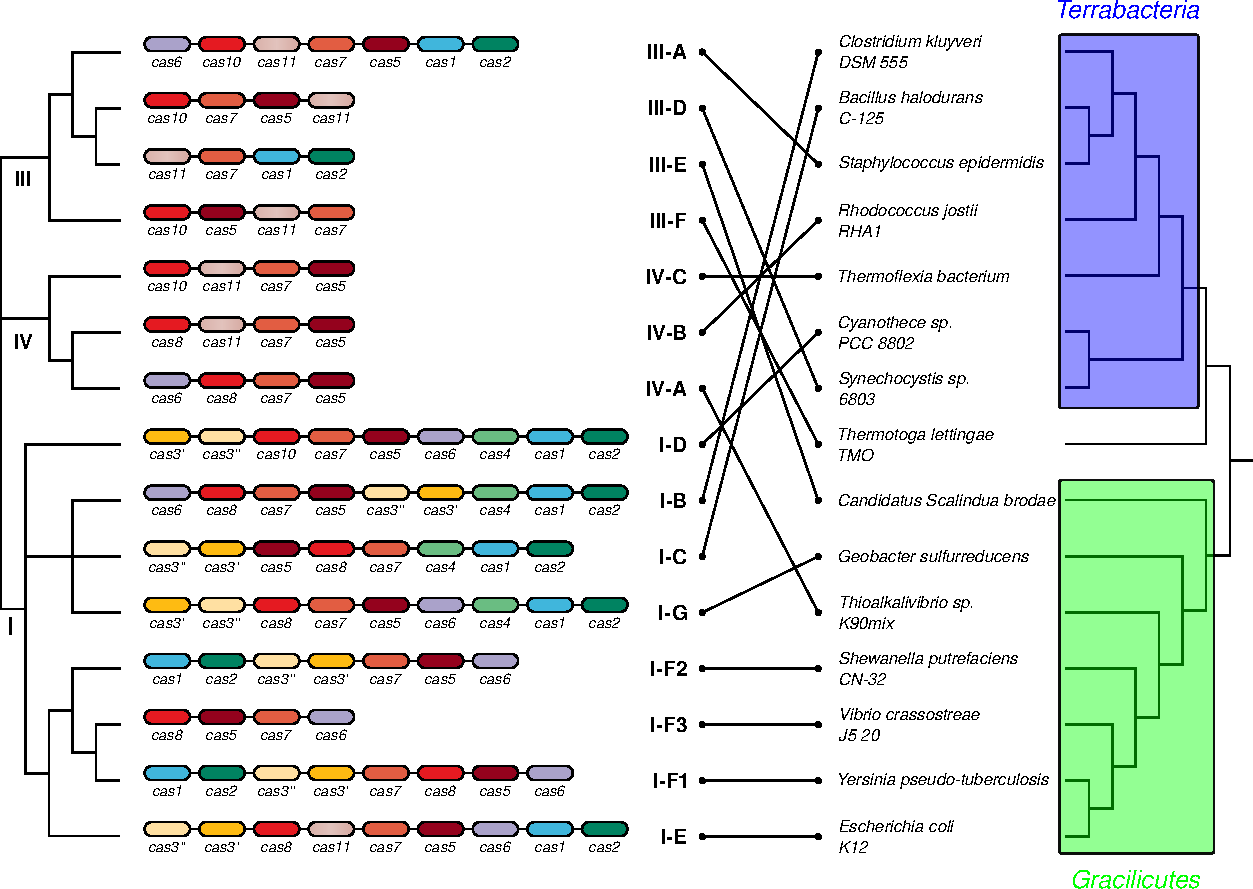
\includegraphics[width=\linewidth]{fig/superdtl/crispr-trees}
    \caption[Dataset of CRISPR-Cas syntenies and their host species]{
        Cas gene syntenies for the 15 considered bacterial species.
        \emph{(Left.)} Phylogeny of Class 1 CRISPR-Cas systems with subtypes names, as presented by~\textcite{Makarova2020EvolutionaryClassificationCRISPR} with our preprocessing of syntenies as described in the text.
        \emph{(Right.)} The species tree based on the topology inferred by~\textcite{Coleman2021RootedPhylogenyResolves} with representation of the two major groups of bacteria, Terrabacteria and Gracilicutes.
        Lines represent the correspondence between the Cas genes syntenies and the species they belong to, illustrating the high incongruence between the topology of the synteny tree and that of the species tree.
        \label{fig:superdtl:crispr-trees}
    }
\end{figure}

We repurposed the phylogenetic tree given in figure~1 of \textcite{Makarova2020EvolutionaryClassificationCRISPR} as our synteny tree.
Some alterations of the syntenies were required to fit the constraints of the model. We considered Cas families Cas1--8 and Cas10--11. Since a part of Cas3, Cas3", can work as a standalone HD nuclease, we split Cas3 into Cas3' and Cas3".
In the paper by~\textcite{Makarova2020EvolutionaryClassificationCRISPR}, Cas10 and Cas8 share the same colour code as they provide similar functions in CRISPR-Cas complexes. Indeed, it was initially believed that Cas8 evolved from Cas10~\parencite{Makarova2011UnificationCasProtein}. Nevertheless, their sequence being extremely divergent, we decided to consider them as not homologous and to conserve separate Cas8 and Cas10 families. Finally, for syntenies with several copies of the same family, we conserved only one copy per synteny. The obtained  Cas gene syntenies are illustrated in the left part of \cref{fig:superdtl:crispr-trees}.

\section{Results}\label{sec:superdtl:results}

\subsection{DTL super-reconciliation settings}

We used {\superdtl} to predict optimal DTL Super-reconciliations for the syntenies and trees depicted in \cref{fig:superdtl:crispr-trees}. Notice that the synteny tree is non-binary and contains three multifurcations, one at the root and two in the subtree of Type I CRISPR-Cas systems. As our algorithm can only be applied to binary trees, we test all possible \enquote{binarizations} of the synteny tree and retain the overall minimal solutions.

We tested different values for the $\delta = \tuple{\costDup, \costHGT, \costLoss}$ cost model, in agreement with a classical assumption that HGTs are less frequent than duplications, which are less frequent than losses. The number of solutions obtained for each setting is given in \cref{tab:superdtl:sol-count}. We observe that the number of solutions decreases as the HGT cost increases, reaching a minimum for $\costHGT=4$, and then increases again. For a given $\costHGT$, the results are largely stable for different $\costDup$ values.

\begin{table}[h]
    \capstart
    \centering
    \setlength{\tabcolsep}{8pt}
    \begin{tabular}{cccccc}
    \toprule
     {\bf $\costHGT$\textbackslash$\costDup$} & {\bf 1} & {\bf 1.5} & {\bf 2} & {\bf 2.5} & {\bf 3}\\
    \midrule
    1 & 1376 & 1376 & 1376 & 1376 & 1376 \\ \midrule
    2 & 132 & 132 & 132 & 132 & 132 \\ \midrule
    3 & 112 & 60 & 60 & 60 & 60 \\ \midrule
    4 & 32 & 32 & 32 & 32 & 48 \\ \midrule
    5 & 288 & 288 & 320 & 32 & 32 \\ \midrule
    6 & 320 & 288 & 288 & 288 & 288 \\
    \bottomrule
    \end{tabular}
    \caption[Number of SuperDTL solutions for various cost settings]{
        Number of solutions obtained by Algorithm {\superdtl} for different values of $\delta = \tuple{\costDup, \costHGT, \costLoss}$, with $\costLoss = 1$.
        \label{tab:superdtl:sol-count}
    }
\end{table}

\begin{figure}[htbp]
    \capstart
    \centering%
    \scalebox{.66}{\colorlet{species background color}{black!10}%
\tikzset{
    x={.95pt},
    y={-1pt},
    species background/.style={
        fill=species background color,
        draw=species background color,
        line width={1pt},
    },
    species label/.style={
        midway,
        anchor=west,
        align=left,
        xshift=5,
    },
    branch/.style={
        draw={#1},
        line width={0.5pt},
    },
    transfer branch/.style={
        branch={#1},
        -Stealth,
    },
    loss/.style={
        draw={#1}, cross out, thick,
        line width={0.5pt},
        inner sep=0pt,
        outer sep=0pt,
        minimum width={3},
        minimum height={3},
    },
    extant gene/.style 2 args={
        circle, fill={#1},
        outer sep=0pt, inner sep=0pt,
        minimum size={3},
        label={
            [font={\color{#1}},
                align=justify,
                inner xsep=4pt, inner ysep=0pt,
                outer xsep=0pt, outer ysep=0pt]
            right:#2
        },
    },
    extant gene/.default={black}{},
    branch node/.style={
        draw={#1}, fill={species background color!50!white},
        align=center,
        font={\color{#1}},
        outer sep=0pt, inner xsep=0pt, inner ysep=2pt,
        line width={0.5pt},
    },
    branch node/.default={black},
    speciation/.style={
        branch node={#1}, rectangle, rounded corners,
        inner xsep=4pt,
        minimum width={8},
        minimum height={8},
    },
    duplication/.style={
        branch node={#1}, rectangle,
        inner xsep=4pt,
        minimum width={8},
        minimum height={8},
    },
    horizontal gene transfer/.style={
        branch node={#1}, chamfered rectangle,
        chamfered rectangle sep={8 / 2.4},
        inner xsep=2pt,
        inner ysep=-1pt,
        minimum width={8},
        minimum height={8},
    },
    gain/.style 2 args={
        branch node={#1}, circle, inner sep=1.5pt,
        label={[font={\strut\scriptsize},xshift=-2pt]right:\color{#1}#2},
    },
    type label/.style 2 args={
        rectangle,
        fill=#1,
        inner sep=0pt,
        outer sep=0pt,
        minimum width=1pt,
        minimum height=6pt,
        label={above:\color{#1}#2},
    },
    group brace/.style={
        decorate,
        decoration={brace},
    },
    group label/.style={
        right=12pt,
        rotate=-90,
        anchor=center,
    },
    clade brace/.style={
        group brace,
        very thick,
    },
    clade label/.style={
        group label,
        font=\bfseries,
    },
}%
\definecolor{reccolor0}{HTML}{000000}%
\definecolor{reccolor1}{HTML}{DB0505}%
\definecolor{reccolor2}{HTML}{0037DB}%
\definecolor{reccolor3}{HTML}{0C8F00}%
\begin{tikzpicture}
% background
\path[species background] (42.17000999999999,269.52636) [rounded corners={4pt}] -- (10,269.52636) -- (10,298.21633) [sharp corners] -- (0,298.21633) -- (0,298.21633) [rounded corners={4pt}] -- (10,298.21633) -- (10,326.90630000000004) [sharp corners] -- (14.0,326.90630000000004) -- (14.0,326.90630000000004) [rounded corners={4pt}] -- (10,326.90630000000004) -- (10,269.52636) [sharp corners] -- (42.17000999999999,269.52636) -- cycle;
\path[species background] (56.17000999999999,163.114845) [rounded corners={4pt}] -- (52.17000999999999,163.114845) -- (52.17000999999999,269.52636) [sharp corners] -- (42.17000999999999,269.52636) -- (42.17000999999999,269.52636) [rounded corners={4pt}] -- (52.17000999999999,269.52636) -- (52.17000999999999,292.21633) [sharp corners] -- (318.94,292.21633) -- (318.94,275.52636) [rounded corners={4pt}] -- (52.17000999999999,275.52636) -- (52.17000999999999,184.30481500000002) [sharp corners] -- (56.17000999999999,184.30481500000002) -- cycle;
\path[species background] (157.22,136.76986) [rounded corners={4pt}] -- (66.17000999999999,136.76986) -- (66.17000999999999,163.114845) [sharp corners] -- (56.17000999999999,163.114845) -- (56.17000999999999,184.30481500000002) [rounded corners={4pt}] -- (66.17000999999999,184.30481500000002) -- (66.17000999999999,246.83639) [sharp corners] -- (158.83341,246.83639) -- (158.83341,213.74642) [rounded corners={4pt}] -- (153.21999999999997,213.74642) -- (153.21999999999997,153.26986) [sharp corners] -- (157.22,153.26986) -- cycle;
\path[species background] (187.72,110.57989) [rounded corners={4pt}] -- (167.22,110.57989) -- (167.22,136.76986) [sharp corners] -- (157.22,136.76986) -- (157.22,153.26986) [rounded corners={4pt}] -- (167.22,153.26986) -- (167.22,167.70983) [sharp corners] -- (318.94,167.70983) -- (318.94,151.01986) [rounded corners={4pt}] -- (183.72,151.01986) -- (183.72,122.07989) [sharp corners] -- (187.72,122.07989) -- cycle;
\path[species background] (213.22,18.18498) [rounded corners={4pt}] -- (197.72,18.18498) -- (197.72,110.57989) [sharp corners] -- (187.72,110.57989) -- (187.72,122.07989) [rounded corners={4pt}] -- (197.72,122.07989) -- (197.72,139.01986) [sharp corners] -- (309.43991,139.01986) -- (309.43991,122.32989) [rounded corners={4pt}] -- (209.22,122.32989) -- (209.22,51.55494) [sharp corners] -- (213.22,51.55494) -- cycle;
\path[species background] (317.82999,0) [rounded corners={4pt}] -- (223.22,0) -- (223.22,18.18498) [sharp corners] -- (213.22,18.18498) -- (213.22,51.55494) [rounded corners={4pt}] -- (223.22,51.55494) -- (223.22,81.48992) [sharp corners] -- (293.15999999999997,81.48992) -- (293.15999999999997,69.98992) [rounded corners={4pt}] -- (289.15999999999997,69.98992) -- (289.15999999999997,28.86996) [sharp corners] -- (317.82999,28.86996) -- cycle;
\path[
                species background,
                rounded corners={4pt},
            ] (317.82999,0) -- (389.26999,0) -- node[species label] (terra-start) {Clostridium\\kluyveri DSM 555} (389.26999,28.86996) -- (317.82999,28.86996);
\path[species background] (318.65999999999997,40.86996) [rounded corners={4pt}] -- (303.15999999999997,40.86996) -- (303.15999999999997,69.98992) [sharp corners] -- (293.15999999999997,69.98992) -- (293.15999999999997,81.48992) [rounded corners={4pt}] -- (303.15999999999997,81.48992) -- (303.15999999999997,110.32989) [sharp corners] -- (326.15999999999997,110.32989) -- (326.15999999999997,81.73992) [rounded corners={4pt}] -- (314.65999999999997,81.73992) -- (314.65999999999997,69.73992) [sharp corners] -- (318.65999999999997,69.73992) -- cycle;
\path[
                species background,
                rounded corners={4pt},
            ] (318.65999999999997,40.86996) -- (389.26999,40.86996) -- node[species label] {Bacillus\\halodurans C-125} (389.26999,69.73992) -- (318.65999999999997,69.73992);
\path[
                species background,
                rounded corners={4pt},
            ] (326.15999999999997,81.73992) -- (389.26998999999995,81.73992) -- node[species label] (firmi-end) {Staphylococcus\\epidermidis} (389.26998999999995,110.32989) -- (326.15999999999997,110.32989);
\path[
                species background,
                rounded corners={4pt},
            ] (309.43991,122.32989) -- (389.26999,122.32989) -- node[species label] {Rhodococcus\\jostii RHA1} (389.26999,139.01986) -- (309.43991,139.01986);
\path[
                species background,
                rounded corners={4pt},
            ] (318.94,151.01986) -- (389.26999,151.01986) -- node[species label] {Thermoflexia\\bacterium} (389.26999,167.70983) -- (318.94,167.70983);
\path[species background] (237.6634,179.70983) [rounded corners={4pt}] -- (168.83341,179.70983) -- (168.83341,213.74642) [sharp corners] -- (158.83341,213.74642) -- (158.83341,246.83639) [rounded corners={4pt}] -- (168.83341,246.83639) -- (168.83341,263.52636) [sharp corners] -- (275.43973,263.52636) -- (275.43973,246.83639000000002) [rounded corners={4pt}] -- (233.6634,246.83639000000002) -- (233.6634,213.74642) [sharp corners] -- (237.6634,213.74642) -- cycle;
\path[
                species background,
                rounded corners={4pt},
            ] (237.6634,179.70983) -- (389.26999,179.70983) -- node[species label] (cyano-start) {Cyanothece\\sp. PCC 8802} (389.26999,213.74642) -- (237.6634,213.74642);
\path[
                species background,
                rounded corners={4pt},
            ] (275.43973,246.83639000000002) -- (389.26999,246.83639000000002) -- node[species label] (terra-end) {Synechocystis\\sp. 6803} (389.26999,263.52636) -- (275.43973,263.52636);
\path[
                species background,
                rounded corners={4pt},
            ] (318.94,275.52636) -- (389.26999,275.52636) -- node[species label] {Thermotoga\\lettingae TMO} (389.26999,292.21633) -- (318.94,292.21633);
\path[species background] (323.94,304.21633) [rounded corners={4pt}] -- (24.0,304.21633) -- (24.0,326.90630000000004) [sharp corners] -- (14.0,326.90630000000004) -- (14.0,326.90630000000004) [rounded corners={4pt}] -- (24.0,326.90630000000004) -- (24.0,386.676235) [sharp corners] -- (28.0,386.676235) -- (28.0,353.306275) [rounded corners={4pt}] -- (24.0,353.306275) -- (24.0,320.90630000000004) [sharp corners] -- (323.94,320.90630000000004) -- cycle;
\path[
                species background,
                rounded corners={4pt},
            ] (323.94,304.21633) -- (389.26999,304.21633) -- node[species label] (gracil-start) {Candidatus\\Scalindua brodae} (389.26999,320.90630000000004) -- (323.94,320.90630000000004);
\path[species background] (303.3299,332.90630000000004) [rounded corners={4pt}] -- (38.0,332.90630000000004) -- (38.0,353.306275) [sharp corners] -- (28.0,353.306275) -- (28.0,386.676235) [rounded corners={4pt}] -- (38.0,386.676235) -- (38.0,406.6462200000001) [sharp corners] -- (118.22000000000003,406.6462200000001) -- (118.22000000000003,395.1462200000001) [rounded corners={4pt}] -- (114.22,395.1462200000001) -- (114.22,361.77626000000004) [sharp corners] -- (303.3299,361.77626000000004) -- cycle;
\path[
                species background,
                rounded corners={4pt},
            ] (303.3299,332.90630000000004) -- (389.26999,332.90630000000004) -- node[species label] (proteo-start) {Geobacter\\sulfurreducens} (389.26999,361.77626000000004) -- (303.3299,361.77626000000004);
\path[species background] (328.94,378.20625000000007) [rounded corners={4pt}] -- (128.22000000000003,378.20625000000007) -- (128.22000000000003,395.1462200000001) [sharp corners] -- (118.22000000000003,395.1462200000001) -- (118.22000000000003,406.6462200000001) [rounded corners={4pt}] -- (128.22000000000003,406.6462200000001) -- (128.22000000000003,472.54115500000006) [sharp corners] -- (143.72,472.54115500000006) -- (143.72,430.67119500000007) [rounded corners={4pt}] -- (139.72000000000003,430.67119500000007) -- (139.72000000000003,394.8962200000001) [sharp corners] -- (328.94,394.8962200000001) -- cycle;
\path[
                species background,
                rounded corners={4pt},
            ] (328.94,378.20625000000007) -- (389.26999,378.20625000000007) -- node[species label] {Thioalkalivibrio\\sp. K90mix} (389.26999,394.8962200000001) -- (328.94,394.8962200000001);
\path[species background] (324.22,406.8962200000001) [rounded corners={4pt}] -- (162.22,406.8962200000001) -- (162.22,430.67119500000007) [sharp corners] -- (143.72,430.67119500000007) -- (143.72,472.54115500000006) [rounded corners={4pt}] -- (162.22,472.54115500000006) -- (162.22,502.63614000000007) [sharp corners] -- (239.82999,502.63614000000007) -- (239.82999,477.63614000000007) [rounded corners={4pt}] -- (235.82999,477.63614000000007) -- (235.82999,435.7661800000001) [sharp corners] -- (324.22,435.7661800000001) -- cycle;
\path[
                species background,
                rounded corners={4pt},
            ] (324.22,406.8962200000001) -- (389.26999,406.8962200000001) -- node[species label] {Shewanella\\putrefaciens CN-32} (389.26999,435.7661800000001) -- (324.22,435.7661800000001);
\path[species background] (328.94,467.44617000000005) [rounded corners={4pt}] -- (249.82999,467.44617000000005) -- (249.82999,477.63614000000007) [sharp corners] -- (239.82999,477.63614000000007) -- (239.82999,502.63614000000007) [rounded corners={4pt}] -- (249.82999,502.63614000000007) -- (249.82999,545.0061000000001) [sharp corners] -- (278.82999,545.0061000000001) -- (278.82999,525.0061000000001) [rounded corners={4pt}] -- (274.82999,525.0061000000001) -- (274.82999,484.13614000000007) [sharp corners] -- (328.94,484.13614000000007) -- cycle;
\path[
                species background,
                rounded corners={4pt},
            ] (328.94,467.44617000000005) -- (389.26999,467.44617000000005) -- node[species label] {Vibrio\\crassostreae J5 20} (389.26999,484.13614000000007) -- (328.94,484.13614000000007);
\path[species background] (318.65999999999997,496.13614000000007) [rounded corners={4pt}] -- (288.82999,496.13614000000007) -- (288.82999,525.0061000000001) [sharp corners] -- (278.82999,525.0061000000001) -- (278.82999,545.0061000000001) [rounded corners={4pt}] -- (288.82999,545.0061000000001) -- (288.82999,573.87606) [sharp corners] -- (312.82999,573.87606) -- (312.82999,545.0061000000001) [rounded corners={4pt}] -- (308.82999,545.0061000000001) -- (308.82999,525.0061000000001) [sharp corners] -- (318.65999999999997,525.0061000000001) -- cycle;
\path[
                species background,
                rounded corners={4pt},
            ] (318.65999999999997,496.13614000000007) -- (389.26999,496.13614000000007) -- node[species label] {Yersinia\\pseudotuberculosis} (389.26999,525.0061000000001) -- (318.65999999999997,525.0061000000001);
\path[
                species background,
                rounded corners={4pt},
            ] (312.82999,545.0061000000001) -- (389.26999,545.0061000000001) -- node[species label] (gracil-end) {Escherichia coli K12} (389.26999,573.87606) -- (312.82999,573.87606);
% clade names
\coordinate (group-labels) at (490,0);
\draw[group brace] (group-labels|-terra-start.north) -- node[group label] {Firmicutes} (group-labels|-firmi-end.south);
\draw[group brace] (group-labels|-cyano-start.north) -- node[group label] {Cyanobacteria} (group-labels|-terra-end.south);
\draw[group brace] (group-labels|-proteo-start.north) -- node[group label] {Proteobacteria} (group-labels|-gracil-end.south);
\coordinate (clade-labels) at (515,0);
\draw[clade brace] (clade-labels|-terra-start.north) -- node[clade label] {Terrabacteria} (clade-labels|-terra-end.south);
\draw[clade brace] (clade-labels|-gracil-start.north) -- node[clade label] {Gracilicutes} (clade-labels|-gracil-end.south);
% gene branches
\path[branch={reccolor0}] (70.17000999999999,173.70983) -- (56.17000999999999,173.70983);
\draw[branch={reccolor0}] (137.22,145.01986) -| (109.69500499999998,167.114845) (109.69500499999998,180.304815) |- node[pos=.25, gain={reccolor0}{1, 2}] {} (158.83341,230.291405);
\path[branch={reccolor1}] (171.22,145.01986) -- (137.22,145.01986) node[type label={reccolor1}{IV}] {};
\draw[branch={reccolor1}] (187.72,116.32989) -| (175.47,140.76986) (175.47,149.26986) |- (318.94,159.364845);
\path[branch={reccolor1}] (203.47,116.32989) -- (187.72,116.32989);
\draw[branch={reccolor1}] (203.47,116.32989) -- (203.47,110.57989);
\draw[branch={reccolor1}] (203.47,116.32989) |- (309.43991,130.674875);
\path[branch={reccolor2}] (227.22,34.869960000000006) -- (213.22,34.869960000000006);
\draw[branch={reccolor2}] (317.82999,14.43498) -| (256.19,22.184980000000003) (256.19,47.55494) |- (293.15999999999997,75.73992);
\path[branch={reccolor2}] (327.82999,14.43498) -- (317.82999,14.43498);
\path[branch={reccolor2}] (308.90999999999997,75.73992) -- (293.15999999999997,75.73992);
\draw[branch={reccolor2}] (308.90999999999997,75.73992) -- (308.90999999999997,81.48992);
\draw[branch={reccolor2}] (308.90999999999997,75.73992) |- (318.65999999999997,55.30494);
\path[branch={reccolor2}] (328.66,55.30494) -- (318.65999999999997,55.30494);
\path[branch={reccolor3}] (336.15999999999997,96.03490500000001) -- (326.15999999999997,96.03490500000001);
\path[branch={reccolor1}] (319.43991,130.674875) -- (309.43991,130.674875);
\draw[branch={reccolor1}] (333.94,130.674875) |- (329.94,130.674875);
\path[branch={reccolor1}] (328.94,159.36484500000003) -- (318.94,159.364845);
\path[branch={reccolor0}] (172.83341,230.291405) -- (158.83341,230.291405);
\draw[branch={reccolor0}] (222.6634,196.728125) -| node[pos=.75, gain={reccolor0}{3', 3", 4}] {} (201.248405,217.74642) (201.248405,242.83639) |- (250.43973,255.181375);
\path[branch={reccolor2}] (247.6634,196.728125) -- (222.6634,196.728125) node[type label={reccolor2}{I}] {};
\draw[branch={reccolor2}] (333.38001,196.728125) |- (329.38000999999997,196.728125);
\draw[branch={reccolor3}] (328.94,255.18137500000003) |- (324.94,255.181375);
\draw[branch={reccolor3}] (314.43991,255.181375) |- (285.43991,255.181375);
\path[branch={reccolor3}] (285.43973,255.181375) -- (250.43973,255.181375) node[type label={reccolor3}{III}] {};
\draw[branch={reccolor3}] (299.93982,255.181375) |- (295.93982,255.181375);
\path[branch={reccolor3}] (328.94,283.871345) -- (276.689775,283.871345);
\path[branch={reccolor3}] (333.94,312.56131500000004) -- (319.689955,312.56131500000004);
\path[branch={reccolor2}] (42.0,369.991255) -- (28.0,369.991255);
\draw[branch={reccolor2}] (303.3299,347.34128000000004) -| (76.11,357.306275) (76.11,382.676235) |- (118.22000000000003,400.8962200000001);
\path[branch={reccolor2}] (313.3299,347.34128000000004) -- (303.3299,347.34128000000004);
\draw[branch={reccolor2}] (327.82999,347.34128000000004) |- (313.3299,347.34128000000004);
\path[branch={reccolor2}] (133.97000000000003,400.8962200000001) -- (118.22000000000003,400.8962200000001);
\draw[branch={reccolor2}] (133.97000000000003,400.8962200000001) -- (133.97000000000003,395.1462200000001);
\draw[branch={reccolor2}] (133.97000000000003,400.8962200000001) |- (143.72,446.13868500000007);
\path[branch={reccolor1}] (338.94,386.5512350000001) -- (328.94,386.5512350000001);
\draw[branch={reccolor2}] (324.22,421.3312000000001) -| (194.774995,443.17119500000007) (194.774995,468.54115500000006) |- (239.82999,494.38614000000007);
\draw[branch={reccolor2}] (230.07999,436.42119500000007) -- (230.07999,430.67119500000007);
\draw[branch={reccolor2}] (230.07999,436.42119500000007) |- (239.82999,483.38614000000007);
\path[branch={reccolor2}] (153.72,446.13868500000007) -- (143.72,446.13868500000007);
\draw[branch={reccolor2}] (230.07999,436.42119500000007) -| (157.97,441.88868500000007) (157.97,450.38868500000007) |- (166.22,455.85617500000006);
\path[branch={reccolor2}] (334.22,421.3312000000001) -- (324.22,421.3312000000001);
\path[branch={reccolor2}] (253.82999,494.38614000000007) -- (239.82999,494.38614000000007);
\draw[branch={reccolor2}] (328.94,475.79115500000006) -| (258.07999,490.13614000000007) (258.07999,498.63614000000007) |- (278.82999,539.2561000000001);
\path[branch={reccolor2}] (269.07999,483.38614000000007) -- (239.82999,483.38614000000007);
\draw[branch={reccolor2}] (269.07999,483.38614000000007) -- (269.07999,480.63614000000007);
\draw[branch={reccolor2}] (269.07999,483.38614000000007) |- (278.82999,530.7561000000001);
\path[branch={reccolor2}] (338.94,475.79115500000006) -- (328.94,475.79115500000006);
\path[branch={reccolor2}] (294.57999,539.2561000000001) -- (278.82999,539.2561000000001);
\draw[branch={reccolor2}] (294.57999,539.2561000000001) -- (294.57999,545.0061000000001);
\draw[branch={reccolor2}] (294.57999,539.2561000000001) |- (318.65999999999997,510.57112000000006);
\path[branch={reccolor2}] (303.07999,530.7561000000001) -- (278.82999,530.7561000000001);
\draw[branch={reccolor2}] (303.07999,530.7561000000001) -- (303.07999,525.0061000000001);
\draw[branch={reccolor2}] (303.07999,530.7561000000001) |- (312.82999,559.44108);
\path[branch={reccolor2}] (328.66,510.57112000000006) -- (318.65999999999997,510.57112000000006);
\path[branch={reccolor2}] (322.82999,559.44108) -- (312.82999,559.44108);
% gene transfers
\draw[transfer branch={reccolor1}] (324.689955,130.67) to[bend right] (328.94,386.5512350000001);
\draw[transfer branch={reccolor2}] (273.521705,209.74642) to[out distance=160pt, out=-90, in=70] (28.0,369.991255);
\draw[transfer branch={reccolor3}] (319.689955,259.431375) to[out=-90, in=90] (319.689955,312.56131500000004);
\draw[transfer branch={reccolor3}] (305.189865,250.931375) to[out=90, in=-110] (326.15999999999997,96.03490500000001);
\draw[transfer branch={reccolor3}] (276.689775,259.431375) to (276.689775,283.871345);
\draw[transfer branch={reccolor2}] (213.579945,347.34) to[bend left=18] (213.22,34.869960000000006);
% events
\node[speciation={reccolor0}] at (109.69500499999998,173.70983) {5, 6, 7, 8, 10, 11};
\node[speciation={reccolor1}] at (175.47,145.01986) {};
\node[loss={reccolor1}] at (203.47,110.57989) {};
\node[speciation={reccolor2}] at (256.19,34.869960000000006) {1, 2, 3', 3",\\4, 5, 6, 7, 8};
\node[extant gene={reccolor2}{1, 2, 3', 3",\\4, 5, 6, 7, 8}] at (329.32999,14.43498) {};
\node[loss={reccolor2}] at (308.90999999999997,81.48992) {};
\node[extant gene={reccolor2}{1, 2, 3', 3",\\4, 5, 7, 8}] at (330.16,55.30494) {};
\node[extant gene={reccolor3}{1, 2, 5, 6,\\7, 10, 11}] at (337.65999999999997,96.03490500000001) {};
\node[extant gene={reccolor1}{5, 7, 8, 11}] at (335.44,130.674875) {};
\node[horizontal gene transfer={reccolor1}] at (324.689955,130.674875) {\phantom{-}};
\node[extant gene={reccolor1}{5, 7, 10, 11}] at (330.44,159.36484500000003) {};
\node[speciation={reccolor0}] at (201.248405,230.291405) {1, 2, 5, 6,\\7, 8, 10, 11};
\node[extant gene={reccolor2}{1, 2, 3', 4,\\5, 6, 7, 10}] at (334.88001,196.728125) {};
\node[horizontal gene transfer={reccolor2}] at (288.521705,196.728125) {1, 2, 3', 3", 4,\\5, 6, 7, 8, 10, 11};
\node[extant gene={reccolor3}{5, 7, 10, 11}] at (330.44,255.18137500000003) {};
\node[horizontal gene transfer={reccolor3}] at (319.689955,255.181375) {\phantom{-}};
\node[horizontal gene transfer={reccolor3}] at (305.189865,255.181375) {\phantom{-}};
\node[horizontal gene transfer={reccolor3}] at (276.689775,255.181375) {\phantom{-}};
\node[extant gene={reccolor3}{5, 7, 10, 11}] at (330.44,283.871345) {};
\node[extant gene={reccolor3}{1, 2, 7, 11}] at (335.44,312.56131500000004) {};
\node[speciation={reccolor2}] at (76.11,369.991255) {1, 2, 3', 3", 4,\\5, 6, 7, 8, 11};
\node[extant gene={reccolor2}{1, 2, 3', 3",\\4, 5, 6, 7, 8}] at (329.32999,347.34128000000004) {};
\node[horizontal gene transfer={reccolor2}] at (213.579945,347.34128000000004) {\phantom{-}};
\node[loss={reccolor2}] at (133.97000000000003,395.1462200000001) {};
\node[extant gene={reccolor1}{5, 6, 7, 8}] at (340.44,386.5512350000001) {};
\node[speciation={reccolor2}] at (194.774995,455.85617500000006) {1, 2, 3', 3",\\5, 6, 7, 8};
\node[loss={reccolor2}] at (230.07999,430.67119500000007) {};
\node[duplication={reccolor2}] at (157.97,446.13868500000007) {};
\node[extant gene={reccolor2}{1, 2, 3',\\3", 5, 6, 7}] at (335.72,421.3312000000001) {};
\node[speciation={reccolor2}] at (258.07999,494.38614000000007) {};
\node[loss={reccolor2}] at (269.07999,480.63614000000007) {};
\node[extant gene={reccolor2}{5, 6, 7, 8}] at (340.44,475.79115500000006) {};
\node[loss={reccolor2}] at (294.57999,545.0061000000001) {};
\node[loss={reccolor2}] at (303.07999,525.0061000000001) {};
\node[extant gene={reccolor2}{1, 2, 3', 3",\\5, 6, 7, 8}] at (330.16,510.57112000000006) {};
\node[extant gene={reccolor2}{1, 2, 3', 3",\\5, 6, 7, 8, 11}] at (324.32999,559.44108) {};
\end{tikzpicture}%}%
    \caption[Most parsimonious scenario for the CRISPR-Cas dataset under SuperDTL]{
        Representation of one of the 32 solutions inferred by Algorithm {\superdtl} reconstructing a DTL evolutionary history of the Class~1 Cas gene synteny dataset illustrated in \cref{fig:superdtl:crispr-trees}.
        Event costs set to $\costLoss=1$, $\costHGT=4$ and $\costDup\in\{1,1.5,2,2.5\}$ yield equal solutions.
        The red, blue, and green parts of the tree reflect the evolution of Cas synteny types IV, I, and III respectively.
        Gains of Cas1+Cas2 and Cas3(Cas3'+Cas3")+Cas4 are illustrated.
        \label{fig:superdtl:crispr-scenario}
    }
\end{figure}

\subsection{An evolutionary scenario}

We analyzed the 32 solutions generated for $\costHGT=4$ and $\costDup\in\{1,1.5,2,2.5\}$. All solutions lead to the same resolution of the three multifurcations in the synteny tree, and the incongruence observed between the species and synteny tree topologies is mainly resolved by inferring six HGTs and one duplication. The 32 solutions only differ from one another by minor variations, such as gene losses located either before or after a speciation or HGT event, which do not change the overall inferred evolutionary history for the Cas gene syntenies.

\Cref{fig:superdtl:crispr-scenario} is a representation of one of these solutions. The evolutionary reconstruction is broadly consistent with the CRISPR-Cas evolution scenario established by \textcite{Koonin2022EvolutionaryPlasticityFunctional}. In both their scenario and ours, the CRISPR-Cas systems emerge from an initial adaptive immune system composed only of Cas genes involved in the effector complex (Cas5--8 and Cas10--11). We see from \cref{fig:superdtl:crispr-scenario} that the CRISPR-Cas emergence is inferred at the root of Terrabacteria. The scenarios diverge on the fact that, in our scenario, Type IV emerges directly from this ancestral adaptive immune system before the acquisition of Cas1 and Cas2 genes, while in \citeauthor{Koonin2022EvolutionaryPlasticityFunctional}'s scenario, Type IV emerges after the acquisition of Cas1 and Cas2 adaptation module genes and loss of several Cas genes.
Aside from this difference, both scenarios are in agreement for Types I and III in terms of gene content in ancestral Cas syntenies. As it appears in \cref{fig:superdtl:crispr-scenario}, Types I and III Cas syntenies emerge from Cyanobacteria after the acquisition of Cas1 and Cas2 by an ancestor of Cyanobacteria. Type I emerges from the branch leading to \emph{Cyanothece sp. PCC 8802} with acquisition of Cas3 and Cas4, while Type III emerges from the branch leading to \emph{Synechocystis sp. 6803} without further gene gains.

Type I was spread to the other bacteria with a HGT to the ancestor of Proteobacteria. According to \textcite{Wang2020EvolutionaryTimelineGenomic}, the Cyanobacteria ancestor is estimated between 2,230 and 3,000 Mya, while the last common ancestor (LCA) of Alpha-, Beta-, and Gammaproteobacteria is estimated between 2,360 and 2,620 Mya. These calibrations make time-plausible the lateral transfer of Type I CRISPR-Cas from the \emph{Cyanothece sp. PCC 8802} branch, close to the Cyanobacteria ancestor, to the LCA of Proteobacteria. A second HGT from \emph{Geobacter sulfurreducens} brought Type I to the Firmicutes \emph{Bacillus halodurans C-125} and \emph{Clostridium kluyveri DSM 555}. Type III was spread across bacteria with a succession of three HGTs, which also seem time-consistent.

The analysis of the synteny evolutionary history across the Proteobacteria subtree shows an unexpected scenario highlighting a limitation of our model. The {\superdtl} algorithm inferred an ancestral synteny duplication before the LCA of \emph{S. putrefaciens}, \emph{V. crassostreae}, \emph{Y. pseudotuberculosis} and \emph{E. coli} resulting in a succession of three consecutive full synteny losses along the branch to the synteny in \emph{E. coli} which is an unlikely evolutionary scenario. An alternative evolutionary scenario would consist in a speciation in place of the duplication, copying the ancestral synteny to an unsampled or extinct species which would later be transferred back to \emph{Escherichia coli}. Such a model of HGT events as combinations of a speciation event outside the species tree (to an unsampled or dead lineage) followed by a transfer back inside the species tree has been described in~\textcite{Szoelloesi2013LateralGeneTransfer}.
This alternative scenario would replace one duplication and three losses with one speciation and one transfer, which yields the same cost under the $\costLoss=1$, $\costHGT=4$ and $\costDup\in\{1,1.5,2,2.5\}$ model but would be less costly for $\costHGT<4$. Consideration of unsampled and dead lineages in the DTL Super-reconciliation will therefore be necessary to infer better synteny evolutionary scenarios.

\section{Conclusion}

We have developed {\superdtl}, the first exact algorithm for inferring most parsimonious evolutionary histories for a set of syntenies, given a phylogenetic tree of the syntenies and a phylogenetic tree of the corresponding species, for an evolutionary model accounting for segmental duplications, gains, losses and HGT events. We only presented the unordered version of the problem in this paper, but the algorithm developed by~\textcite{Delabre2020EvolutionSegmentalDuplications} for the ordered version of the DL Super-reconciliation model can also be extended to the DTL Super-reconciliation model. However, as rearrangements are not considered in the model, a DT or DTL Super-reconciliation only exists if extant gene orders are pairwise consistent, which is a strong constraint, not verified, for example, in the case of the Cas gene syntenies of \cref{fig:superdtl:crispr-trees}. Considering a unifying model accounting for both DTL and rearrangement events remains a challenge. The analysis of the synteny evolutionary scenario in Proteobacteria emphasized the need in DTL Super-reconciliation model to infer HGT to and from unsampled or extinct species to produce more realistic evolutionary scenarios.
In addition, in order to avoid the unjustified constraint of having all genes at the root of the tree, we allowed for gene gains, which has been essential for the analysis of Cas gene syntenies. Although we defined the general evolutionary model in a way allowing for segmental gains (i.e. gains of a group of genes), we only considered single gene gains in our algorithm. An extension is however possible and may be considered for future work.

The reconstruction of an evolutionary history for Cas gene syntenies  using {\superdtl} provides a first attempt to reconcile the evolutionary scenario of Cas syntenies in the context of the evolution of bacterial species. However, several improvements could be brought to the considered Cas synteny dataset to better reconstruct its evolutionary history. First, we excluded archaea from our dataset while several studies show evidence for an emergence of CRISPR-Cas systems from archaeal species followed by horizontal transfers to bacteria. This is supported by the fact that most considered archaea have a complete CRISPR-Cas system while only part of bacteria have one. In fact, as of the latest update from January 21, 2021 of the CRISPRCasdb database\footnote{Available at \url{https://crisprcas.i2bc.paris-saclay.fr/MainDb/StrainList}}~\parencite{Pourcel2020CRISPRCasdbSuccessorCRISPRdb}, 70.64\% of analyzed archaeal species versus 36.27\% of analyzed bacteria had a complete CRISPR-Cas system.
A phylogenetic dating approach could also be used to produce a dated phylogeny of prokaryotes and to constrain HGT events.
A larger dataset with species sampling representing the diversity of archaea and bacteria with dated phylogeny and Cas synteny tree based on synteny content and sequence divergence is required to further elucidate the evolutionary history of the CRISPR-Cas system in prokaryotes.
